\documentclass[11pt]{article}
\usepackage[reqno]{amsmath}
\usepackage{amssymb}
\usepackage{epsf}
\usepackage{epsfig}
\usepackage{rotate}
\usepackage{hyperref}
\newcommand{\ol}{\overline}
\newcommand{\ul}{\underline}
\newcommand{\vb}{\verbatim}
\newcommand{\bi}{\begin{itemize}}
\newcommand{\ei}{\end{itemize}}
\newcommand{\be}{\begin{enumerate}}
\newcommand{\ee}{\end{enumerate}}
\newcommand{\noi}{\noindent}
\newcommand{\ro}{{\bf R}^1 }
\newcommand{\rn}{{\bf R}^n }
\newcommand{\lra}{\Longrightarrow}
\newcommand{\qlq}{\quad\lra\quad}
\newcommand{\bul}{\bullet}
\newcommand{\llim}{\lim\limits}
\newcommand{\xc}{_{x\to c}}
\newcommand{\nin}{_{n\to\infty}}
\newcommand{\pb}{\parbox{1in}}
\newcommand{\pbof}{\parbox[t]{1.5in}}
\newcommand{\pbt}{\parbox[t]{2in}}
\newcommand{\pbff}{\parbox[t]{4in}}
\newcommand{\rot}{\rotate[r]}
\newcommand{\ep}{\epsffile}
\newcommand{\eps}{\epsilon}
\newcommand{\beqa}{\begin{eqnarray}}
\newcommand{\eeqa}{\end{eqnarray}}
\newcommand{\non}{\nonumber}
\newcommand{\di}{D^{-1}}
\newcommand{\lint}{\int\limits}
\newcommand{\bmat}{\begin{matrix}}
\newcommand{\emat}{\end{matrix}}
\newcommand{\bal}{\begin{align}}
\newcommand{\eal}{\end{align}}
\setcounter{MaxMatrixCols}{20}
\newcommand{\bpm}{\begin{pmatrix}}
\newcommand{\epm}{\end{pmatrix}}
\newcommand{\bvm}{\begin{vmatrix}}
\newcommand{\evm}{\end{vmatrix}}
\newcommand{\bfx}{{\bf x}}
\newcommand{\bfa}{{\bf A}}
\newcommand{\fx}{f(\bfx)}
\newcommand{\pr}{\partial}
\newcommand{\pf}{\pr \fx}
\newcommand{\grad}{\nabla \fx}
\newcommand{\hx}{\bf H(x)}



\oddsidemargin=0in
\evensidemargin=0in
\textwidth=6.5in
\topmargin=0in
\headsep=.25in
\headheight=.25in
\textheight=9.25in
\topskip=0in
\voffset=-0.5in
\epsfxsize=1in

\begin{document}
\pagestyle{myheadings}
\markright{Math Camp 2012: Calculus}
\parskip=6pt
\thispagestyle{empty}
\renewcommand{\thefootnote}{\fnsymbol{footnote}}

\begin{centering}
{\Large \bf Math Camp 2012:\\[9pt]
 Calculus}\\[18pt]
August 2012\\[36pt]
\end{centering}


\noi {\bf Topics}\footnote{These notes were prepared by Jacob Montgomery. Much of the material and examples for
this lecture are taken from Harvard ``Math (P)refresher'' class notes
whose authors are listed
\href{http://people.hmdc.harvard.edu/~mathpre/mathnotes/lectures/index.html}{here}
and \textit{A Mathematical Primer for Social Statistics} by John Fox.}:
\bi
\item Limits
\bi
\item The limits of a function
\item Continuity
\item The limit of a series
\ei
\item Change we can believe in
\bi
\item Derivatives 
\item Higher-Order Derivatives 
\item  Maxima and Minima 
\item  Composite Functions 
\item  The Chain Rule,  Derivatives of Exp and Ln 
\item  L'Hospital's Rule
\ei
\item The area under a curve
\bi
\item The Indefinite Integral: The Antiderivative 
\item The Definite Integral: The Area under the Curve 
\item Integration by Substitutions 
\item Integration by Parts
\ei
\item Calculus in higher dimensions
\bi
\item Partial Derivatives
\item Partial Derivatives of Higher Order
\item Multidimensional Integrals
\item Calculus in vector and matrix form
\item First order conditions
\item Second order conditions and the Hessian
\item Global or local?
\ei
\ei


\section{Limits}

\begin{center}
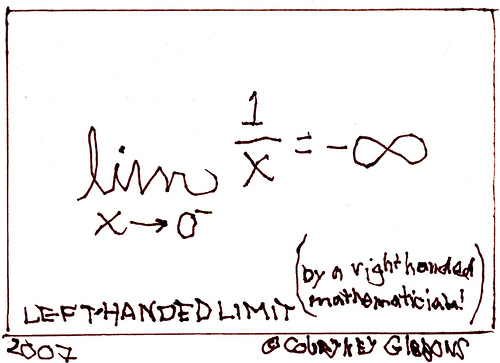
\includegraphics[width=3in]{Limits}
\end{center}



\bi
\item We're often interested in determining if a function $f$ approaches
some number $L$ as its independent variable $x$ moves to some
number $c$ (usually 0 or $\pm\infty$).  If it does, we say that $f(x)$
approaches $L$ as $x$ approaches $c$, or $\lim\xc f(x)=L$.
\item {\bf Limit of a function}.  Let $f$ be defined at
each point in some open interval containing the point $c$, although
possibly not defined at $c$ itself.  Then $\llim\xc f(x)=L$ if for
any (small positive) number $\eps$, there exists a corresponding
number $\delta>0$ such that if $0<|x-c|<\delta$, then
$|f(x)-L|<\eps$.

\item Examples:
  \be
  \item $\llim\xc k = k$
  \item $\llim\xc x = c$
  \item \parbox[t]{1.5in}{$\llim_{x\to 0} |x| = 0$}\pb{\,  {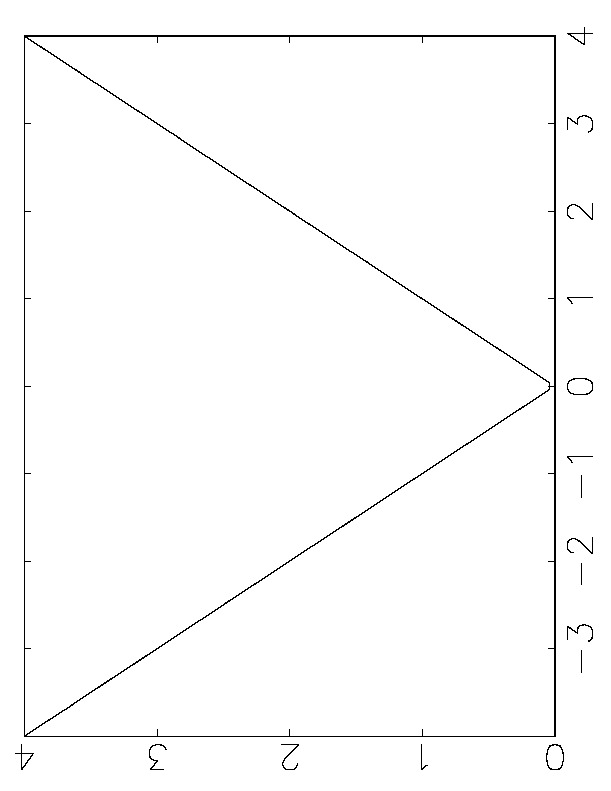
\includegraphics[width=1in, angle = 270]{abs2}}}
  \item \parbox[t]{1.5in}{$\llim_{x\to 0}
\left(1+\frac{1}{x^2}\right)=\infty$} \pb{\,  {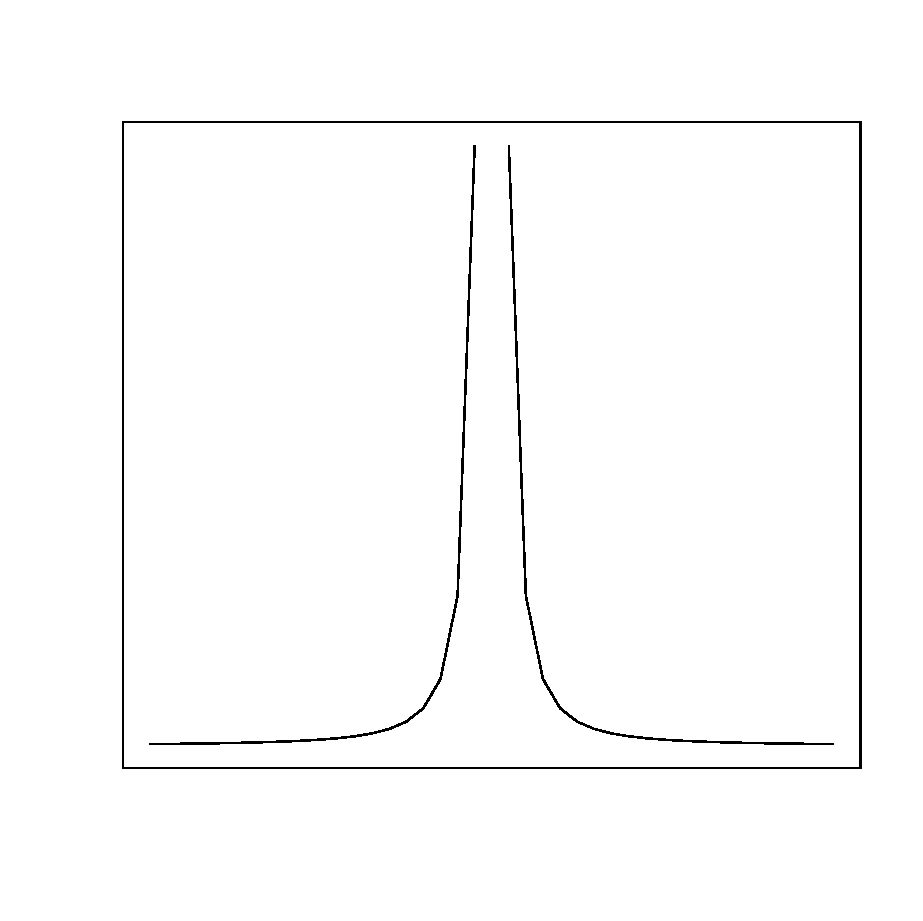
\includegraphics[width=1in]{this}}}
  \ee
\item Uniqueness: $\llim\xc f(x)=L$ and $\llim\xc f(x)=M \lra L=M$
\item Properties: Let $f$ and $g$ be functions with $\llim\xc
f(x)=A$ and $\llim\xc g(x)=B$.
  \be
  \item $\llim\xc[f(x)+g(x)]=\llim\xc f(x)+ \llim\xc g(x)= A+B$
  \item $\llim\xc \alpha f(x) = \alpha \llim\xc f(x) = \alpha A$
  \item $\llim\xc f(x) g(x) = [\llim\xc f(x)][\llim\xc g(x)]= A B$
  \item $\llim\xc \frac{f(x)}{g(x)} = \frac{\llim\xc f(x)}{\llim\xc
g(x)} = \frac{A}{B}$, provided $B\ne 0$
  \ee
\item Examples:
  \be
  \item $\llim_{x\to 2} (2x-3) = 2\llim_{x\to 2} x- 3\llim_{x\to 2} 1
= 2\times 2 - 3\times 1 = 1$
  \item $\llim\xc x^n = [\llim\xc x]\cdots[\llim\xc x] = c\cdots c =
c^n$
  \ee
\item Other types of limits:
  \be
  \item \pbt{\bf Right-hand limit:} $\llim_{x\to c^+} f(x) = L$, if $c<x<c+\delta \lra |f(x)-L|<\eps$\\
\parbox[t]{2.75in}{Example:  $\llim_{x\to 0^+} \sqrt{x} = 0$}\pb{\,
  {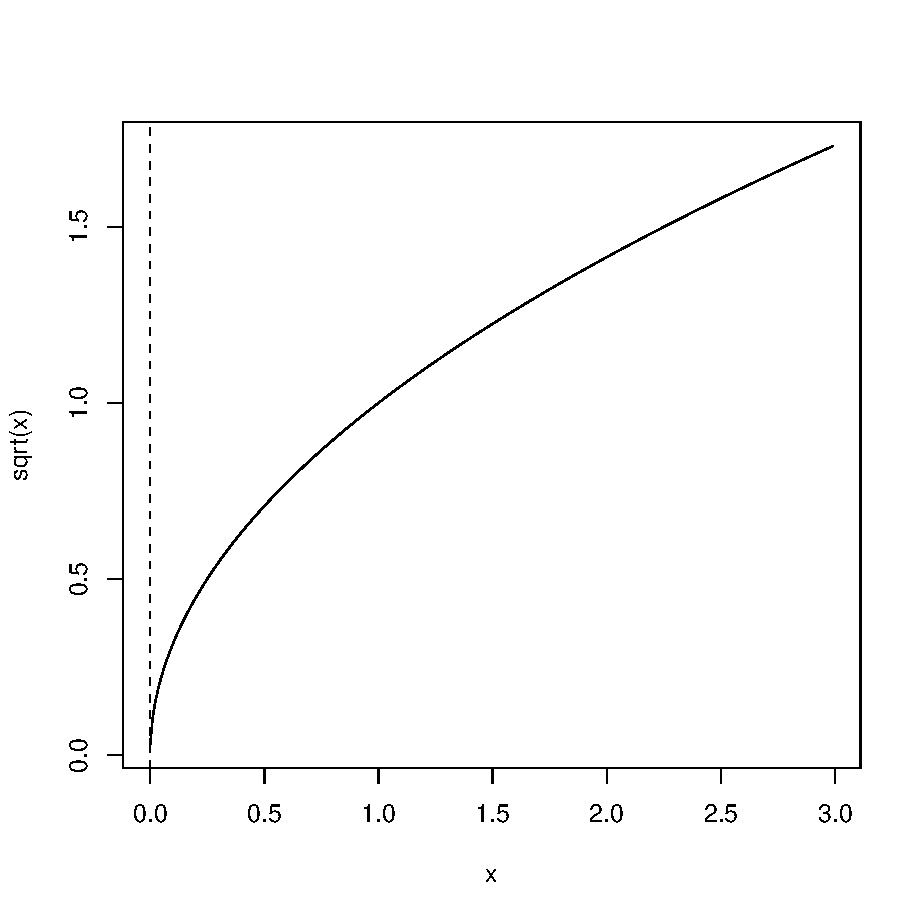
\includegraphics[width=1in]{sqrtJ}}}
  \item \pbt{\bf Left-hand limit:}  $\llim_{x\to c^-} f(x) = L$, if
$c-\delta<x<c \lra |f(x)-L|<\eps$
  \item \pbt{\bf Infinity:} $\llim_{x\to \infty} f(x)=L$, if $x>N
\lra |f(x)-L|<\eps$
  \item \pbt{\bf $-$Infinity:} $\llim_{x\to -\infty} f(x)=L$, if $x<-N
\lra |f(x)-L|<\eps$\\
\parbox[t]{2.75in}{Example:  $\llim_{x\to \infty} 1/x = \llim_{x\to
-\infty} 1/x= 0$}\pb{\,  {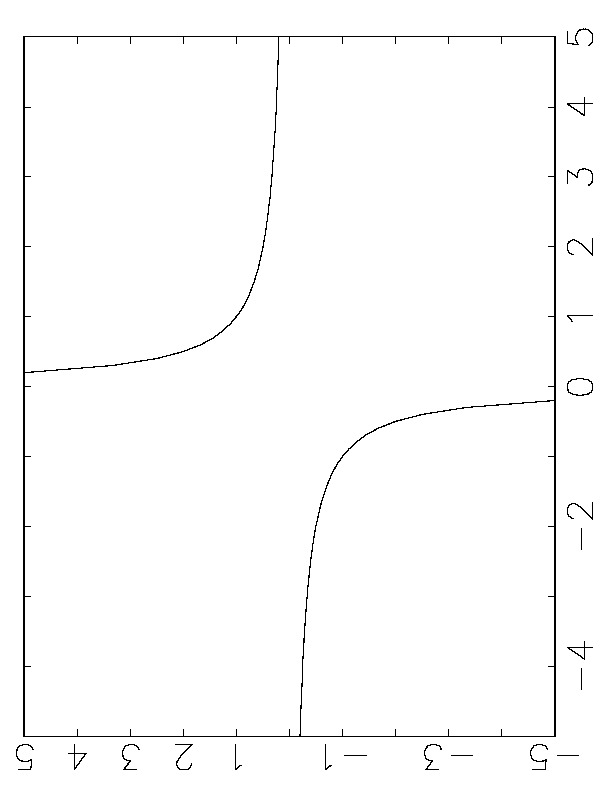
\includegraphics[width=1in]{1ovrxJ}}}
  \ee

\item \textbf{Caution}: In some situations, you will not be able to
  calculate a limit.  For instance, $\lim_{x\to \infty}\frac{x}{-x}$.
  The numerator is headed towards $\infty$ while the denominator is
  headed towards $-\infty$.  In this case the limit does not exist.
  In other circumstances, the limit may exist but additional steps
  need to be taken.  \ei


\section{Continuity}
\bi
\item {\bf Continuity}: Suppose that the domain of the function $f$
includes an open interval containing the point $c$.  Then $f$ is
continuous at $c$ if $\llim\xc f(x)$ exists and if $\llim\xc f(x)=f(c)$.
Further, $f$ is continuous on an open interval $(a,b)$ if it is
continuous at each point in the interval.
\item Examples: Continuous functions.\\
   \parbox[t]{1.5in}{\hfill$f(x)=\sqrt{x}\quad$}\pb{\,  {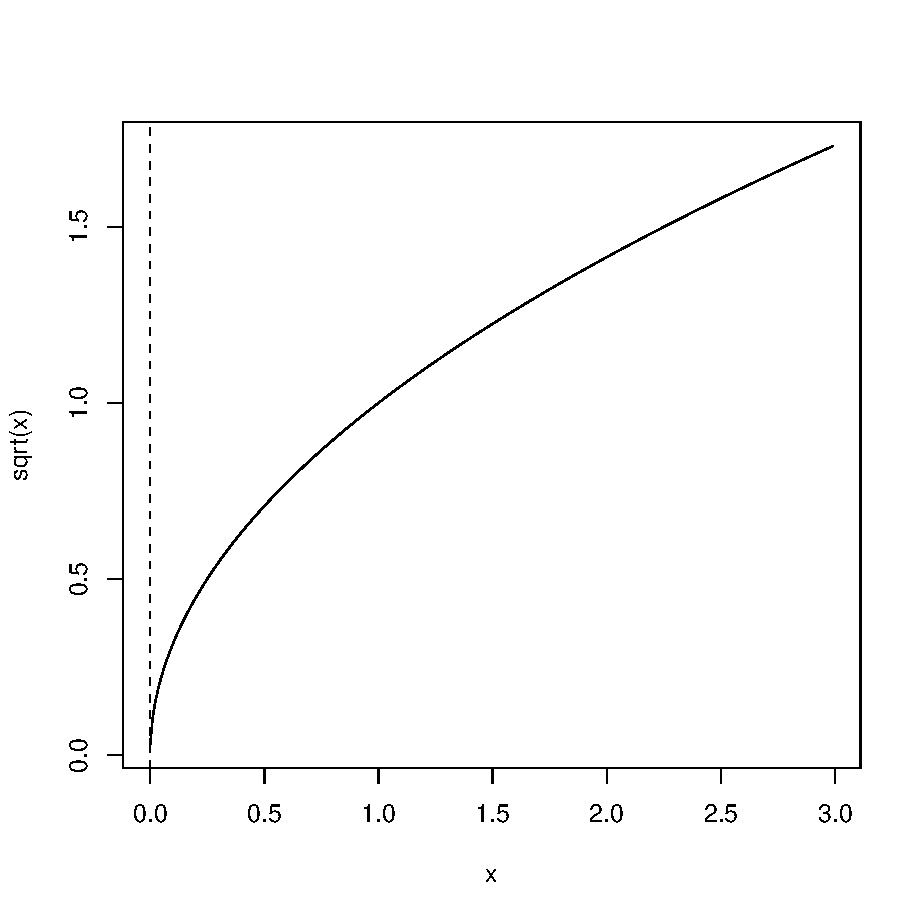
\includegraphics[width=1in, angle = 270]{sqrtJ}}}
   \parbox[t]{1.5in}{\hfill$f(x)=e^x\quad$}\pb{\,  {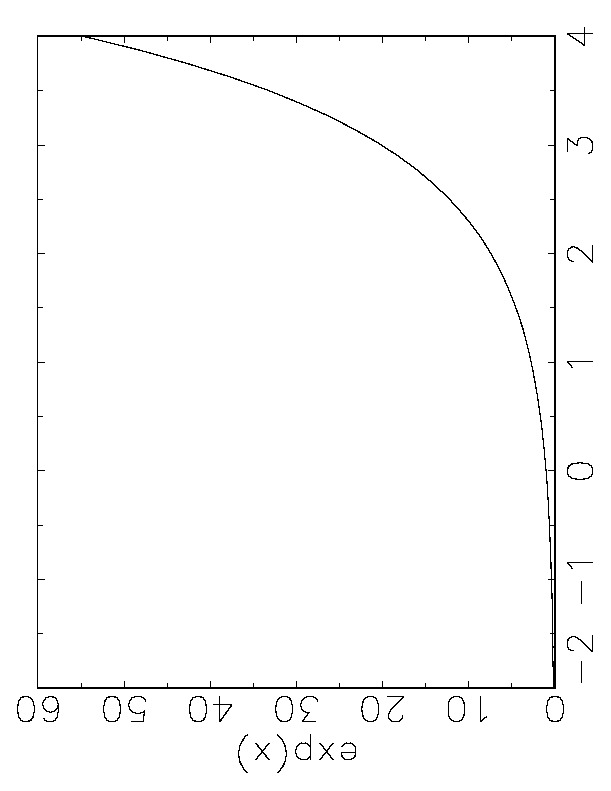
\includegraphics[width=1in, angle = 270]{expJ}}}
\item Examples: Discontinuous functions.\\
   \parbox[t]{1.5in}{\hfill$f(x)=\mbox{floor}(x)\quad$}\pb{\,  {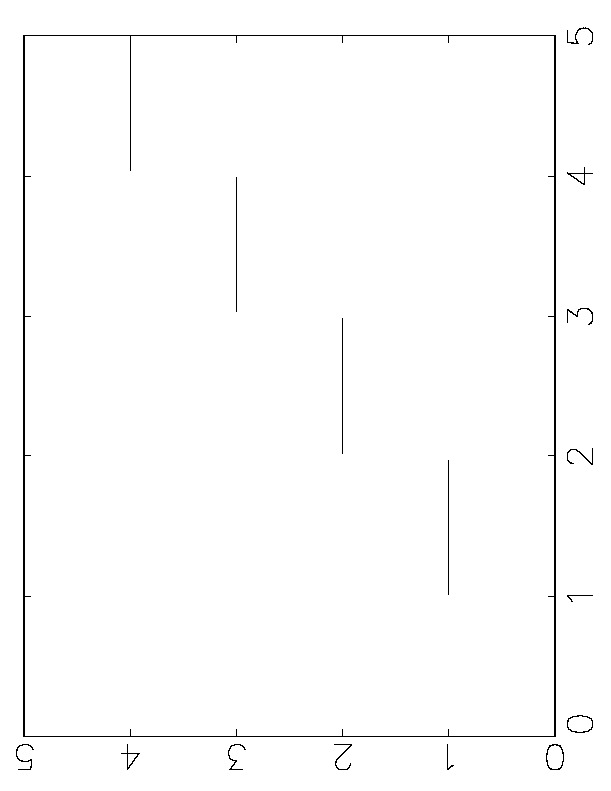
\includegraphics[width=1in, angle = 270]{floorJ}}}
   \parbox[t]{1.5in}{\hfill$f(x)=1+\frac{1}{x^2}\quad$}\pb{\,  {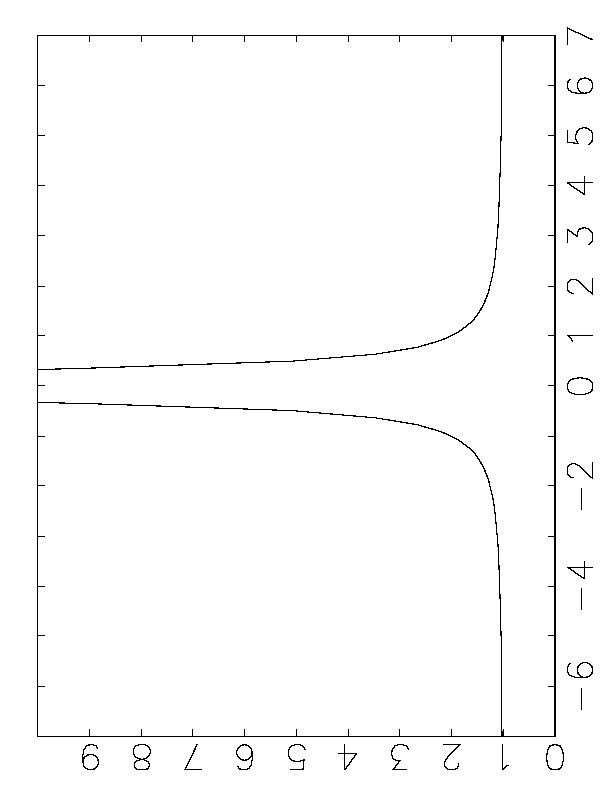
\includegraphics[width=1in, angle = 270]{1p1ovrx2J}}}
\item Properties:
  \be
  \item If $f$ and $g$ are continuous at point $c$, then $f+g$, $f-g$, $f g$,
   $|f|$, and $\alpha f$ are continuous. $f/g$ is continuous, provided
   $g(c)\ne 0$.
  \item {\bf Boundedness}: If $f$ is continuous on the closed bounded
   interval $[a,b]$, then there is a number $K$ such that $|f(x)|\le K$
   for each $x$ in $[a,b]$.
  \item {\bf Max/Min}: If $f$ is continuous on the closed bounded
   interval $[a,b]$, then $f$ has a maximum and a minimum on $[a,b]$,
   possibly at the end points.
  \item The range of a closed bounded interval $[a,b]$ under a
   continuous function $f$ is also a closed bounded interval $[m,M]$.
  \ee
\ei

% \section{Continuity}
% \bi
% \item {\bf Continuity}: Suppose that the domain of the function $f$
% includes an open interval containing the point $c$.  Then $f$ is
% continuous at $c$ if $\llim\xc f(x)$ exists and if $\llim\xc f(x)=f(c)$.
% Further, $f$ is continuous on an open interval $(a,b)$ if it is
% continuous at each point in the interval.
% \item Examples: Continuous functions.\\
%    \parbox[t]{1.5in}{\hfill$f(x)=\sqrt{x}\quad$}\pb{\,  {\includegraphics[width=1in, angle = 270]{sqrt.eps}}}
%    \parbox[t]{1.5in}{\hfill$f(x)=e^x\quad$}\pb{\,  {\includegraphics[width=1in, angle = 270]{exp.eps}}}
% \item Examples: Discontinuous functions.\\
%    \parbox[t]{1.5in}{\hfill$f(x)=\mbox{floor}(x)\quad$}\pb{\,  {\includegraphics[width=1in, angle = 270]{floor.eps}}}
%    \parbox[t]{1.5in}{\hfill$f(x)=1+\frac{1}{x^2}\quad$}\pb{\,  {\includegraphics[width=1in, angle = 270]{1p1ovrx2.eps}}}
% \item Properties:
%   \be
%   \item If $f$ and $g$ are continuous at point $c$, then $f+g$, $f-g$, $f g$,
%    $|f|$, and $\alpha f$ are continuous. $f/g$ is continuous, provided
%    $g(c)\ne 0$.
%   \item {\bf Boundedness}: If $f$ is continuous on the closed bounded
%    interval $[a,b]$, then there is a number $K$ such that $|f(x)|\le K$
%    for each $x$ in $[a,b]$.
%   \item {\bf Max/Min}: If $f$ is continous on the closed bounded
%    interval $[a,b]$, then $f$ has a maximum and a minimum on $[a,b]$,
%    possibly at the end points.
%   \item The image of a closed bounded interval $[a,b]$ under a
%    continuous function $f$ is also a closed bounded interval $[m,M]$.
%   \ee
% \ei


% % \subsection{Graphing Functions}
% % \bi
% % \item Know your function. How? \emph{Graph your function.}
% % \item A picture is worth a thousand words.
% %   \be
% %   \item Is the function increasing or decreasing?  Over what part of the
% % domain?
% %   \item How ``fast" does it increase or decrease?
% %   \item Are there global or local maxima and minima?  Where?
% %   \item Are there inflection points?
% %   \item Is the function continuous?
% %   \item Is the function differentiable?
% %   \item Does the function tend to some limit?
% %   \item Other questions related to the substance of the problem at hand.
% %   \ee
% % \ei


% \subsection{Finding Roots}
% \bi
% \item Solving for variables is especially important when we want to find
% the {\bf roots} of an equation: those values of variables that cause an
%  equation to equal zero.
% \item Especially important in finding equilibria and in doing maximum
% likelihood estimation.
% \item Procedure: Given $y=f(x)$, set $y=0$.  Solve for $x$.
% \item There may be multiple roots.
% \item \parbox[t]{4.75in}{For quadratic equations $ax^2+bx+c=0$, use
% $x=\frac{-b\pm\sqrt{b^2-4ac}}{2a}$.}
% %\epsfxsize=1in\parbox{1in}{\, {\includegraphics[width=.9in, angle = 270]{roots.eps}}}
% \item Examples:
%   \be
%   \item $f(x)=3x+2 \qlq 3x+2=0 \qlq x=-\frac{2}{3}$
%   \item $f(x)=e^{-x}-10 \qlq e^{-x}-10=0 \qlq e^{-x}=10 \qlq x=-\ln(10)$
%   \item $f(x)=x^2+3x-4=0 \qlq x=\{1,-4\}$.
%   \ee
% \ei

% \subsection{Quadratic Functions}
% The quadratic equation
% FOIL


% \subsection{}

\subsection{Sequences}
\bi

\item A {\bf sequence} $\{y_n\}=\{y_1, y_2, y_3, \ldots, y_n\}$ is an
ordered set of real numbers, where $y_1$ is the first term in the
sequence and $y_n$ is the $n$th term.  Generally, a sequence extends to
$n=\infty$. We can also write the sequence as $\{y_n\}^\infty_{n=1}$.
\item Examples:
  \be
  \item \parbox[t]{3in}{$\{y_n\}=\left\{ 2-\frac{1}{n^2} \right\} = \left\{ 1,
\frac{7}{4}, \frac{17}{9}, \frac{31}{16}, \ldots \right\}$}\pb{\,
{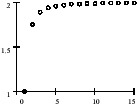
\includegraphics[width=1.5in]{limitJ}}}
  \item \parbox[t]{3in}{$\{y_n\}=\left\{ \frac{n^2+1}{n} \right\} = \left\{ 2,
\frac{5}{2}, \frac{10}{3}, \ldots \right\}$}\pb{\,  {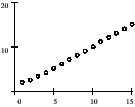
\includegraphics[width=1.5in]{unboundJ}}}
  \item \parbox[t]{3in}{$\{y_n\}=\left\{ (-1)^n \left(1-\frac{1}{n}\right) \right\}
 = \{ 0, \frac{1}{2}, -\frac{2}{3}, \frac{3}{4}, \ldots \}$}\pb{\,  {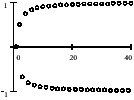
\includegraphics[width=1.5in]{altrnateJ}}}
  \ee
\item Think of sequences like functions.  Before, we had $y=f(x)$ with
$x$ specified over some domain.  Now we have $\{y_n\}=\{f(n)\}$ with
$n=1,2,3,\ldots$.
\item Three kinds of sequences:
  \be
  \item Sequences like 1 above that converge to a limit.
  \item Sequences like 2 above that increase without bound.
  \item Sequences like 3 above that neither converge nor increase
without bound --- alternating over the number line.
  \ee
\item Boundedness and monotonicity:
  \be
  \item {\bf Bounded}: if $|y_n|\le K$ for all $n$
  \item {\bf Monotone Increasing}: $y_{n+1}>y_n$ for all $n$
  \item {\bf Monotone Decreasing}: $y_{n+1}<y_n$ for all $n$
  \ee
\item {\bf Subsequence}: choose an infinite collection of entries from
$\{ y_n \}$, retaining their order.
\ei

\subsection{The Limit of a Sequence}
\bi
\item We're often interested in whether a sequence {\bf converges}
to a {\bf limit}.  Limits of sequences are conceptually similar to the
limits of functions addressed in the previous lecture.
\item {\bf Definition: (Limit of a sequence)}.  The sequence $\{y_n\}$
has the limit $L$, that is $\llim\nin y_n =L$, if for any
$\eps>0$ there is an integer $N$ (which depends on $\eps$) with
the property that $|y_n -L|<\eps$ for each $n>N$.  $\{y_n\}$ is said
to converge to $L$.  If the above does not hold, then $\{y_n\}$
diverges.
\item Examples:
  \be
  \item $\llim\nin \left\{ 2-\frac{1}{n^2} \right\} = 2$
  \item \parbox[t]{2in}{$\llim\nin \left\{ \frac{4^n}{n!} \right\} = 0$}
\pb{\,  {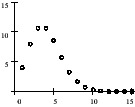
\includegraphics[width=1.5in]{limit2J}}}
  \ee
\item Uniqueness: If $\{y_n\}$ converges, then the limit $L$ is unique.
\item Properties: Let $\llim\nin y_n = A$ and
$\llim\nin z_n =B$.  Then
  \be
  \item $\llim\nin [\alpha y_n + \beta z_n]=\alpha A+\beta B$
  \item $\llim\nin y_n z_n = A B$
  \item $\llim\nin \frac{y_n}{z_n} = \frac{A}{B}$, provided $B\ne 0$
  \ee

\item Finding the limit of a sequence in $\rn$ is similar to that in
$\ro$.
\item {\bf Limit of a sequence of vectors.} The sequence
of vectors $\bf \{ y_n \}$ has the limit $\bf L$, that is
$\llim_{n\to\infty} {\bf y_n}={\bf L}$, if for any $\eps$ there is an
integer $N$ where $\bf ||y_n-L||<\eps$ for each $n>N$.  The sequence
of vectors $\bf \{ y_n\}$ is said to converge to the vector $\bf L$ --- and
the distances between $\bf y_n$ and $\bf L$ converge to zero.

\item Think of each coordinate of the vector $\bf y_n$ as being part of
its own sequence over $n$.  Then a sequence of vectors in $\rn$
converges if and only if all $n$ sequences of its components converge.\\
Examples:
  \be
  \item The sequence $\{ y_n \}$ where $y_n=\left( \frac{1}{n},
2-\frac{1}{n^2} \right)$ converges to $(0,2)$.
  \item The sequence $\{ y_n \}$ where $y_n=\left( \frac{1}{n}, (-1)^n
\right)$ does not converge, since $\left\{ (-1)^n \right\}$ does not
converge.
  \ee
\ei


\section{Change we can believe in}

\begin{center}
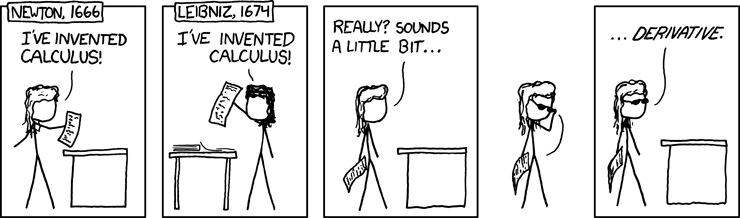
\includegraphics[width=6in]{newton}
\end{center}

\noi Although you will be using matrix notation and linear algebra on a
pretty regular basis (mostly in your statistics classes), encounters with basic
concepts from calculus will be a daily event in your methods training.  In the
case of derivatives, you will primarily be using them to:
\bi
\item Find the maximum and minimum values of specific functions
  including utility and likelihood functions; 
\item Derive a probability density function given its cumulative
  density function
\ei

\noi This probably doesn't mean much to you at the moment.  But what
they have in common is that we are trying to understand a certain
property of a function -- the rate of change.  Usually we want to find
when the rate of change is zero, as that indicates either a maximum or
minimum.  These concepts were developed in the 17th century to
understand physical motion.  If a function describes the location of
a baseball flying through the air, the first derivative describes the
velocity of the ball, and the second derivative represents the
acceleration.

\subsection{Derivative}
\bi
\item The derivative of $f$ at $x$ is its rate of change at $x$ ---
i.e., how much $f(x)$ changes with a change in $x$.\\
\bi
\item For a line, the derivative is the slope.\\
\item  For a curve, the derivative is the tangent line at $x$.
\ei

\item {\bf Derivative}:  Let $f$ be a function whose domain includes an
open interval containing the point $x$.  The derivative of $f$ at
$x$ is given by
\beqa
f'(x) &=&\llim_{h\to 0} \frac{f(x+h)-f(x)}{(x+h)-x}\nonumber\\
      &=&\llim_{h\to 0} \frac{f(x+h)-f(x)}{h}\nonumber
\eeqa

\item Don't succumb to the temptation to take this equation as a given
  without any understanding.  This idea is over 400 years old now, and
  is not beyond your abilities to understand.

Imagine that you want to calculate how a function changes between time
period 1 and period 2.  With a little thought we would calculate
this as:

$$ m = \frac{f(x_2) - f(x_1)}{x_2 - x_1}$$

This is same ``rise over run'' calculation we used to calculate the
slope of a line in the first lecture.  If we set $h = x_2 - x_1$ and
$x = \frac{x_1 + x_2}{2}$ then
we can re-parametrize this as:

$$m = \frac{f(x+h/2) - f(x-h/2)}{h}$$
$$ = \frac{f(x+h) - f(x)}{h}$$

What we want to calculate is the ``instantaneous'' rate of change.
That is, we want to know the rate of change as $x_1$ and $x_2$ get
closer and closer together such that time period between when we
measure them moves towards zero.  In other words, what happens as $h$
gets very close to to zero.  This is the conceptual leap that it takes a
genius like Newton to discover, but which we can accept with a bit of
thought.

\item If $f'(x)$ exists at a point $x$, then $f$ is said to be {\bf
differentiable} at $x$.  Similarly, if $f'(x)$ exists for every point
along an interval, then $f$ is differentiable along that interval.  For
$f$ to be differentiable at $x$, $f$ must be both continuous and
``smooth'' at $x$.  The process of calculating $f'(x)$ is called {\bf
differentiation}.

\item For historical reasons, there are multiple notations for
  derivatives.  
  \be
  \item \pbt{$y'$, $f'(x)$} (Prime or Lagrange Notation)
    \item \pbt{$\frac{dy}{dx}$, $\frac{df}{dx}(x)$} (Leibniz's Notation)
  \ee

\item Examples:
  \be
  \item $f(x)=c$\\
   $f'(x)=\llim_{h\to 0} \frac{f(x+h)-f(x)}{h}
   =\llim_{h\to 0} \frac{c-c}{h}
   =\llim_{h\to 0} 0 = 0$
  \item \pbff{$f(x)=x$\\
   $f'(x)=\llim_{h\to 0} \frac{(x+h)-x}{h}
   =\llim_{h\to 0} 1 = 1$}
   \pb{\,  {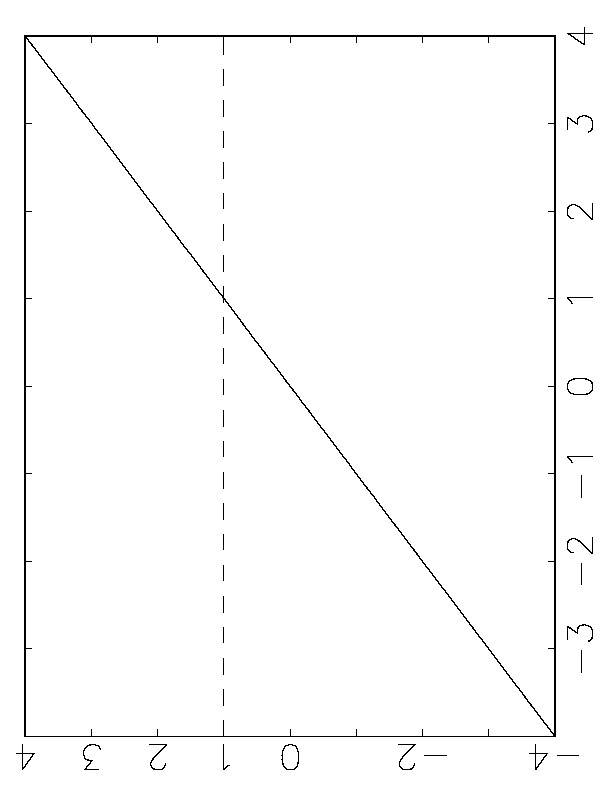
\includegraphics[width=1in, angle = 270]{derivxJ}}}
  \item \pbff{$f(x)=x^2$\\
   $f'(x)=\llim_{h\to 0} \frac{(x+h)^2-x^2}{h}
   =\llim_{h\to 0}\frac{2xh+h^2}{h}
   =\llim_{h\to 0} (2x + h) = 2x$}
   \pb{\,  {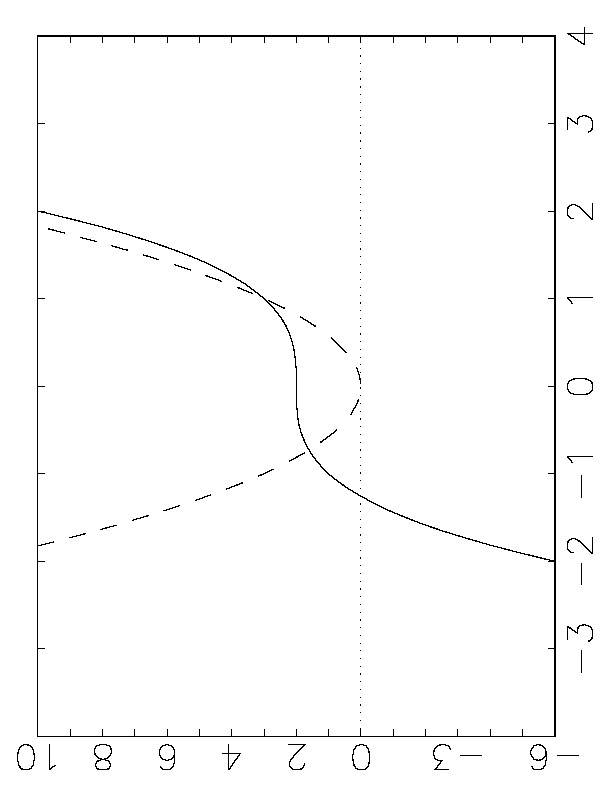
\includegraphics[width=1in, angle = 270]{derivx2J}}}
  \item \pbff{$f(x)=x^3$\\
   $f'(x) = \llim_{h\to 0}\frac{(x+h)^3-x^3}{h}
   = \llim_{h\to 0}\frac{3x^2 h +3xh^2 + h^3}{h}\\
   = \llim_{h\to 0}\left(3x^2 + 3xh+h^2\right)
   = 3x^2$}
   \pb{\,  {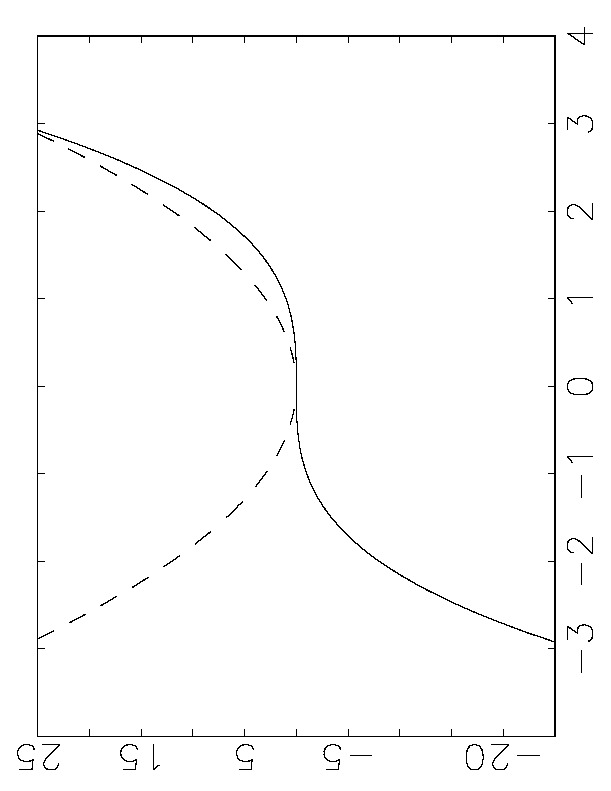
\includegraphics[width=1in, angle = 270]{derivx3J}}}
  \ee

\item \textbf{Aside:} A function is \textit{monotonically increasing}
  in a domain if it has a positive derivative over that domain.
  Likewise, it is \textit{monotonically decreasing} if it has a negative
  derivative.

\item \textbf{Existence}: $f'(x)$ at some particular value of $x$
  exits iff $f(x)$ is continuous at that value of $x$.  $f'(x)$ exists
  for all values of $x$ iff $f(x)$ is continuous at all values of $x$
  in the domain of $f(x)$.  In other words, there must be no point
  where the right-hand derivative and the left-hand derivative are
  different.  The basic test is ``can you draw the function without
  lifting your pencil.''  The classic case where this does not work
  are:

\be
\item $$f(x) = |x|$$
\item $$ f(x) = \frac{1}{x-1}$$
\item $$f(x) = 1, x \in [0,1]$$
$$ f(x) = 0,  x > 1 \mbox{ or } x<0$$
\ee 


\item Doing this calculation for every function is cumbersome, and
  sometimes difficult.  Fortunately, hundreds of mathematical graduate
  students and professors have developed several ``rules'' that help
  us calculate derivatives quickly.  All of these rules come with
  proofs, but for our purposes we usually just memorize them and use
  them.  The first (and easiest) is that the derivative of a constant
  is zero.


\textbf{Properties of derivatives}:  Suppose that $f$ and $g$ are
differentiable at $x$ and that $\alpha$ is a constant.  Then the
functions $f\pm g$, $\alpha f$, $f g$, and $f/g$ (provided $g(x)\ne 0$)
are also differentiable at $x$.  Additionally,\\
  \pbt{\bf Power rule:} $[x^k]' = k x^{k-1}$  \\
  \pbt{\bf Sum rule:} $[f(x)\pm g(x)]' = f'(x)\pm g'(x)$ \\
  \pbt{\bf Constant rule:} $[\alpha f(x)]' = \alpha f'(x)$ \\
  \pbt{\bf Product rule:} $[f(x)g(x)]' = f'(x)g(x)+f(x)g'(x)$\\
  \pbt{\bf Quotient rule:} $[f(x)/g(x)]' =
\frac{f'(x)g(x)-f(x)g'(x)}{[g(x)]^2}$, $g(x)\ne 0$\\


\item Examples:
  \be
  \item $f(x)=3x^2+2x^{1/3}$\\
   $f'(x)=(3x^2)'+(2x^{1/3})'
   =3(2x)+2(\frac{1}{3}x^{-2/3})
   =6x+\frac{2}{3}x^{-2/3}$\\
  \item $f(x)=(x^3)(2x^4)$\\
   $f'(x)=(x^3)'(2x^4)+(x^3)(2x^4)'
   =(3x^2)(2x^4)+(x^3)(8x^3)
   =6x^6+8x^6=14x^6$\\
   or\\
   $f'(x)=(2x^7)'=14x^6$\\
  \item $f(x)=\frac{x^2+1}{x^2-1}$\\
   $f'(x)=\frac{(x^2+1)'(x^2-1)-(x^2+1)(x^2-1)'}{(x^2-1)^2}
   =\frac{2x(x^2-1)-(x^2+1)2x}{(x^2-1)^2}
   =\frac{-4x}{(x^2-1)^2}$
  \ee
\ei

\subsection{Higher-order derivatives}
\bi
\item One conceptual leap you need to make is that $f'(x)$ is just
  another function of $x$.  An input value for $x$ gives an output
  value determined by $f'(x)$.  For some people it might help to change
  the name so that $h(x) = f'(x)$.  The important thing to understand
  is that just as $f(x)$ can have a derivative, $f'(x)$ can also have
  have a derivative.  

\item  We can keep applying the differentiation process to functions
that are themselves derivatives.  The derivative of $f'(x)$ with respect
to $x$, would then be $$f''(x)=\llim_{h\to 0}\frac{f'(x+h)-f'(x)}{h}$$
and so on.  Similarly, the derivative of $f''(x)$ would be denoted
$f'''(x)$.
\item  \pbt{{\bf First derivative}:} $f'(x)$, $y'$, $\frac{df(x)}{dx}$,
$\frac{dy}{dx}$\\
\pbt{{\bf Second derivative}:} $f''(x)$, $y''$, $\frac{d^2f(x)}{dx^2}$,
$\frac{d^2y}{dx^2}$\\
\pbt{{\bf $\bf n$th derivative}:}  $\frac{d^nf(x)}{dx^n}$,
$\frac{d^ny}{dx^n}$

\item Example: $f(x)=x^3$, $f'(x)=3x^2$, $f''(x)=6x$, $f'''(x)=6$, $f''''(x)=0$

\item Example: $$f(x) = 4x^4 + 12x^2+x-2$$
$$f'(x) = 16x^3 - 24x + 1$$
$$f''(x) = 48x^2 - 24$$
$$f'''(x) = 96x$$
$$f''''(x) = 96$$
$$f'''''(x) = 0$$

\ei



\subsection{Maxima and minima}
\bi
\item The first derivative $f'(x)$ identifies whether the function
 $f(x)$ at the point $x$ is
   \be
   \item \parbox[t]{2in}{\bf Increasing:} $f'(x)>0$
   \item \parbox[t]{2in}{\bf Decreasing:} $f'(x)<0$
   \item \parbox[t]{2in}{{\bf Extremum/Saddle}:} $f'(x)=0$
   \ee


\item Examples:
   \be
   \item \parbox[t]{2in}{$f(x)=x^2+2$, $f'(x)=2x$}
    \pb{\,  {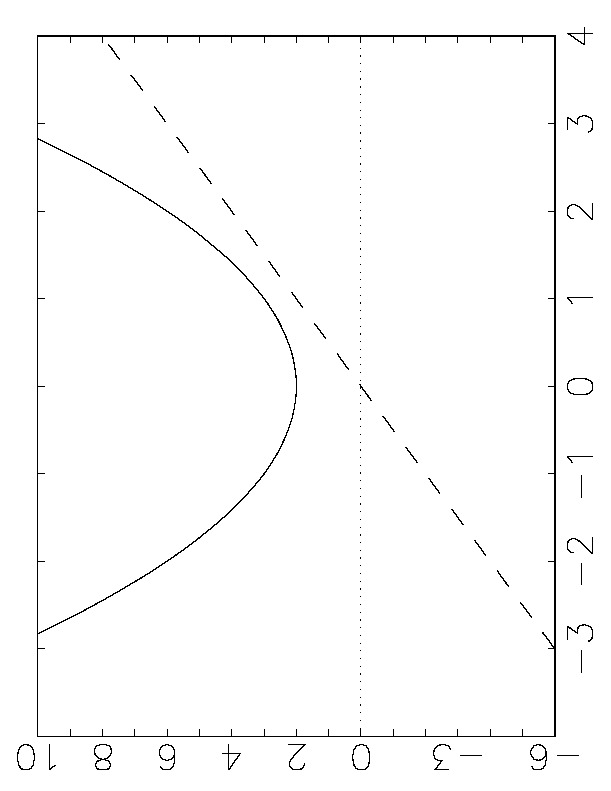
\includegraphics[width=1in, angle = 270]{deriv1J}}}
   \item \parbox[t]{2in}{$f(x)=x^3+2$, $f'(x)=3x^2$}
    \pb{\,  {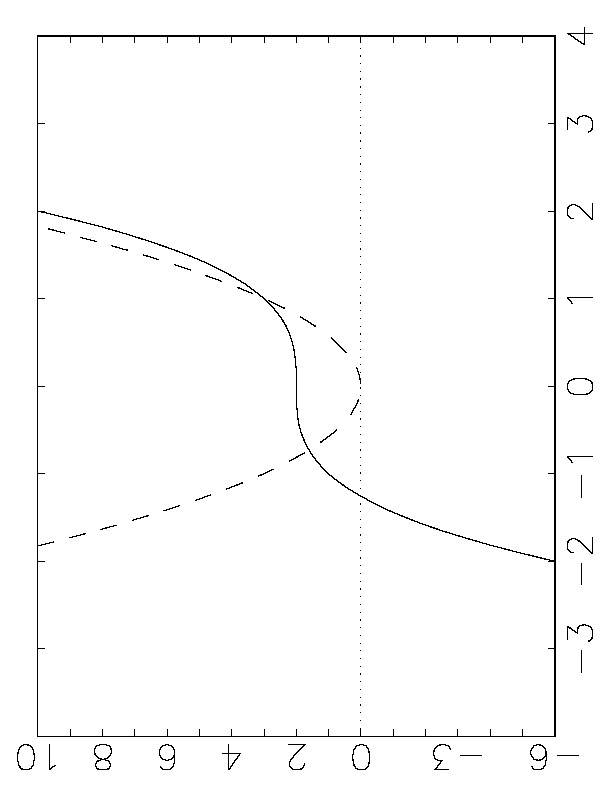
\includegraphics[width=1in, angle = 270]{deriv2J}}}
   \ee


\item The second derivative $f''(x)$ identifies whether the
function $f(x)$ at the point $x$ is
  \be
  \item \pbt{\bf Concave down:} $f''(x)<0$
  \item \pbt{\bf Concave up:} $f''(x)>0$
  \ee

\item {\bf Maximum (Minimum)}: $x_0$ is a {\bf local} maximum (minimum)
      if $f(x_0)>f(x)$ ($f(x_0)<f(x))$ for all $x$ within some open
      interval containing $x_0$.  $x_0$ is a {\bf global} maximum
      (minimum) if $f(x_0)>f(x)$ ($f(x_0)<f(x))$ for all $x$ in the
      domain of $f$.

\item {\bf Critical points}: Given the function $f$ defined over domain
      $D$, all of the following are critical points:
      \be
      \item Any interior point of $D$ where $f'(x)=0$.
      \item Any interior point of $D$ where $f'(x)$ does not exist.
      \item Any endpoint that is in $D$.
      \ee

The maxima and minima will be a subset of the critical points.

\item  Combined, the first and second derivatives can tell us whether a
 point is a maximum or minimum of $f(x)$. \\[6pt]
 \pbt{\bf Local Maximum:} $f'(x)=0$ and $f''(x)<0$\\
 \pbt{\bf Local Minimum:} $f'(x)=0$ and $f''(x)>0$\\
 \pbt{\bf Need more info:} $f'(x)=0$ and $f''(x)=0$

\item {\bf Global Maxima and Minima}. Sometimes no global max or min
 exists --- e.g., $f(x)$ not bounded above or below.  However, three
 situations where we can fairly easily identify global max or min.
   \be
   \item {\bf Functions with only one critical point.} If $x_0$ is a local
    maximum of $f$ and it is the only critical point, then it is a global
    maximum.
   \item {\bf Globally concave up or concave down functions.}  If $f''$
    is never zero, then there is at most one critical point, which is a
    global maximum if $f''<0$ and a global minimum if $f''>0$.
   \item {\bf Functions over closed and bounded intervals} must have both
    a global maximum and a global minimum.
   \ee

\item Examples:
  \be
    \item \parbox[t]{1.25in}{$f(x)=x^2+2$\\$f'(x)=2x$\\$f''(x)=2$}
     \parbox[t]{4.5in}{$f'(x)=2x=0$ at $x=0$ and it is the only critical
     point.  Checking
     $f''(x)$, we see that $f''(x)>0$ for all $x$.  Therefore, $x=0$ is a
     global minimum.  We could also have noted that $f''(x)$ is globally
     concave up and concluded that $x=0$ is a global minimum.\\[6pt]}
    \item \parbox[t]{1.25in}{$f(x)=x^3+2$\\$f'(x)=3x^2$\\$f''(x)=6x$}
     \parbox[t]{4.5in}{$f'(x)=0$ at $x=0$ and it is the only critical point.
     However, $f''(0)=0$, so we need more information to determine if $x=0$
     is a maximum, minimum, or saddle.  If we examined either the graph
     or values of $f''(x)$ around $x=0$, we would find that $x=0$ is in fact a
     saddle point.  Since $f(x)$ is unbounded above or below, there are
     no maxima or minima.\\}
     \item \parbox[t]{3in}{$f(x)=|x^2-1|$, $x\in [-2,2]$\\[6pt]
      $f'(x)=\left\{
      \begin{array}{rll}
      2x & & -2<x<-1, 1<x<2 \\
      -2x& & -1<x<1
      \end{array}
      \right.$\\
      $f''(x)=\left\{
      \begin{array}{rll}
      2 & & -2<x<-1, 1<x<2 \\
      -2& & -1<x<1
      \end{array}
      \right.$\\
      \epsfxsize=1.25in
      {\,  {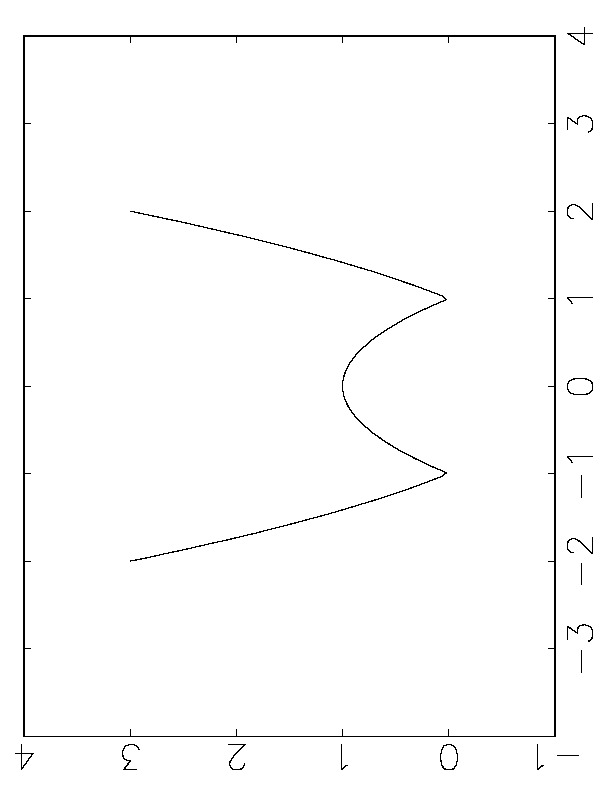
\includegraphics[width=1in, angle = 270]{absx2m1J}}}}
      \parbox[t]{2.75in}{There are five critical points.  The two endpoints
      are $(-2,3)$ and $(2,3)$.  $f'(x)$ is not defined for $x=\pm 1$, so
      $(-1,0)$ and $(1,0)$ are also critical points.  Additionally, $f'(x)=0$
      for $x=0$, so $(0,1)$ is a critical point.  Since $f''(0)$ is negative,
      $(0,1)$ is a local maximum.  Comparing $f(x)$ for these five points, we
      conclude that $(-2,3)$ and $(2,3)$ are global maxima and $(-1,0)$ and
      $(1,0)$ are global minima.}
  \ee
\ei

\subsection{Chain rule}
\bi
\item {\bf Composite functions} are formed by substituting one function
into another and are denoted by $$(f\circ g)(x)=f[g(x)]$$  To form
 $f[g(x)]$, the range of $g$ must be contained (at least in part) within
the domain of $f$. The domain of $f\circ g$ consists of all the points
in the domain of $g$ for which $g(x)$ is in the domain of $f$.
\item Examples:
  \be
  \item \pbt{$f(x)=\ln x$,}  $0<x<\infty$\\
  \pbt{$g(x)=x^2$} $-\infty<x<\infty$\\
  \pbt{$(f\circ g)(x)=\ln x^2$,} $-\infty<x<\infty - \{0\}$\\
  \pbt{$(g\circ f)(x)=[\ln x]^2$,} $0<x<\infty$\\
  Notice that $f\circ g$ and $g\circ f$ are not the same functions.
  \item \pbt{$f(x)=4+\sin x$,} $-\infty<x<\infty$\\
  \pbt{$g(x)=\sqrt{1-x^2}$,} $-1\le x\le 1$\\
  \pbt{$(f\circ g)(x)=4+\sin \sqrt{1-x^2}$,} $-1\le x\le 1$\\
  $(g\circ f)(x)$ does not exist, since the range of $f$, $[3,5]$, has no
points in common with the domain of $g$.
  \ee

\item {\bf Chain Rule}:  Let $y=f(z)$ and $z=g(x)$.  Then, $y=(f\circ
g)(x)=f[g(x)]$ and the derivative of $y$ with respect to $x$ is
$$\frac{d}{dx} \{ f[g(x)] \} = f'[g(x)] g'(x)$$ which can also be
written as $$\frac{dy}{dx}=\frac{dy}{dz} \frac{dz}{dx}$$ (Note: the
above does not imply that the $dz$'s cancel out, as in fractions.  They
are part of the derivative notation and have no separate existence.)
The chain rule can be thought of as the derivative of the ``outside"
times the derivative of the ``inside," remembering that the derivative
of the outside function is evaluated at the value of the inside
function.

\item {\bf Generalized Power Rule}:  If $y=[g(x)]^k$, then
$dy/dx=k[g(x)]^{k-1}g'(x)$.

\item Examples:
  \be
  \item Find $dy/dx$ for $y=(3x^2+5x-7)^6$.
Let $f(z)=z^6$ and $z=g(x)=3x^2+5x-7$.  Then, $y=f[g(x)]$ and
\beqa
\frac{dy}{dx}&=& f'(z) g'(x)\non\\
             &=& \left(6z^5\right) (6x+5)\non\\
             &=& 6\left(3x^2+5x-7\right)^5 (6x+5)\non
\eeqa
  \item Find $dy/dx$ for $y=\sin(x^3+4x)$.
(Note: the derivative of $\sin x$ is $\cos x$.)  Let $f(z)=\sin z$ and
$z=g(x)=x^3+4x$.  Then, $y=f[g(x)]$ and
\beqa
\frac{dy}{dx}&=& f'(z) g'(x)\non\\
             &=& \left(\cos z\right) (3x^2+4)\non\\
             &=& \cos\left(x^3+4x\right) \left(3x^2+4\right)\non
\eeqa
  \ee
\ei

\subsection{Derivatives of Exp and Ln}
\bi
\item {\bf Derivatives of Exp}:
  \be
  \item $\frac{d}{dx}\alpha e^x = \alpha e^x$
  \item $\frac{d^n}{dx^n} \alpha e^x = \alpha e^x$
  \item $\frac{d}{dx}e^{u(x)}= e^{u(x)} u'(x)$
  \ee

\item Examples:  Find $dy/dx$ for
  \be
  \item \pbof{$y=e^{-3x}$}\pbff{Let $u(x)=-3x$.  Then $u'(x)=-3$
and $dy/dx=-3e^{-3x}$.}
  \item \pbof{$y=e^{x^2}$}\pbff{Let $u(x)=x^2$.  Then $u'(x)=2x$
and $dy/dx=2xe^{x^2}$.}
  \item \pbof{$y=e^{\sin 2x}$}\pbff{Let $u(x)=\sin 2x$.  Then
$u'(x)=2\cos 2x$ and $dy/dx=(2\cos 2x) e^{\sin 2x}$.}
  \ee

\item {\bf Derivatives of Ln}:
  \be
  \item $\frac{d}{dx} \ln x = \frac{1}{x}$
  \item $\frac{d}{dx} \ln x^k = \frac{d}{dx} k \ln x = \frac{k}{x}$
  \item $\frac{d}{dx} \ln u(x) = \frac{u'(x)}{u(x)}\quad$  (by the chain rule)
  \ee

\item Examples:  Find $dy/dx$ for
  \be
  \item \pbof{$y=\ln(x^2+9)$}\pbff{Let $u(x)=x^2+9$.  Then
$u'(x)=2x$ and $dy/dx=u'(x)/u(x)=2x/(x^2+9)$.}
  \item \pbof{$y=\ln(\ln x)$}\pbff{Let $u(x)=\ln x$.  Then
$u'(x)=1/x$ and $dy/dx=1/(x\ln x)$.}
  \item \pbof{$y=(\ln x)^2$}\pbff{Use the generalized power rule.
 $dy/dx=(2\ln x)/x$.}
  \item \pbof{$y=\ln e^x$}\pbff{(We know that $\ln e^x=x$ and
that $dx/dx=1$, but let's double check.)  Let $u(x)=e^x$.  Then
$u'(x)=e^x$ and $dy/dx=u'(x)/u(x)=e^x/e^x=1$.}
  \ee

\item For any positive base $b$, $\frac{d}{dx} b^x = (\ln
b)\left(b^x\right)$.

\ei

\subsection{L'Hospital's Rule}
\bi
\item In studying limits, we saw that $\llim\xc f(x)/g(x) = \left(\llim\xc
f(x)\right)/\left(\llim\xc g(x)\right)$, provided that $\llim\xc g(x)\ne
0$, which will cause the limit to be unbounded.
\item If both $\llim\xc f(x)=0$ and $\llim\xc g(x)=0$, then we get an
{\bf indeterminate form} of the type $0/0$ as $x\to c$.  However, we can
still analyze such limits using L'Hospital's rule.
\item {\bf L'Hospital's Rule}:  Suppose $f$ and $g$ are differentiable
on $a<x<b$ and that either
  \be
  \item $\llim_{x\to a^+} f(x)=0$ and $\llim_{x\to a^+} g(x)=0$, or
  \item $\llim_{x\to a^+} f(x)=\pm\infty$ and $\llim_{x\to a^+} g(x)=\pm\infty$\
  \ee
Suppose further that $g'(x)$ is never zero on $a<x<b$ and that
$$\llim_{x\to a^+} \frac{f'(x)}{g'(x)}=L$$ then
$$\llim_{x\to a^+} \frac{f(x)}{g(x)}=L$$

\item Examples:  Use L'Hospital's rule to find the following limits:
  \be
  \item \pbof{$\llim_{x\to 0^+}\frac{\ln(1+x^2)}{x^3}$}
  \pbff{Let $f(x)=\ln(1+x^2)$ and $g(x)=x^3$.  Then $f'(x)=2x/(1+x^2)$
and $g'(x)=3x^2$.  Using L'Hospital's rule, $\llim_{x\to 0^+}
\frac{2x/(1+x^2)}{3x^2} = \llim_{x\to 0^+} \frac{2}{3x(1+x^2)} = \infty$.}
  \item \pbof{$\llim_{x\to  0^+} \frac{e^{1/x}}{1/x}$}
  \pbff{Let $f(x)=e^{1/x}$ and $g(x)=1/x$.  Then
$f'(x)=-\frac{1}{x^2}e^{1/x}$ and $g'(x)=-1/x^2$.  Using L'Hospital's
rule, $\llim_{x\to  0^+} \frac{-\frac{1}{x^2}e^{1/x}}{-1/x^2}=\llim_{x\to  0^+}
e^{1/x}=\infty$.}
  \item \pbof{$\llim_{x\to 2} \frac{x-2}{(x+6)^{1/3}-2}$}
   \pbff{Let $f(x)=x-2$ and $g(x)=(x+6)^{1/3}-2$.  Then $f'(x)=1$ and
$g'(x)=\frac{1}{3}(x+6)^{-2/3}$.  Using L'Hospital's rule, $\llim_{x\to 2}
\frac{1}{\frac{1}{3}(x+6)^{-2/3}} = 3(8)^{2/3}=12$.}
  \ee
\ei


\subsection{Newton-Raphson and Taylor Series}
\bi

\item For various reasons, derivatives can be difficult to write down.
  This is particularly true in the kinds of higher-dimensional
  settings we discuss below.  The \emph{Newton-Raphson} and
  \emph{Taylor Series expansion} approaches are sometimes used in
  these situations to find the value when $f'(x)= 0$ or at some value
  $x_1$ respectively.

\item For reasons of time, we are not going to cover this in great
  detail, but more advanced students may want to carefully look at
  section 6.4.2 in the book and/or consult more advanced calculus
  texts.  In particular, you are very likely to see a Taylor series
  expansion in the next couple of years.
\ei


\section{The area under a curve}

\begin{center}
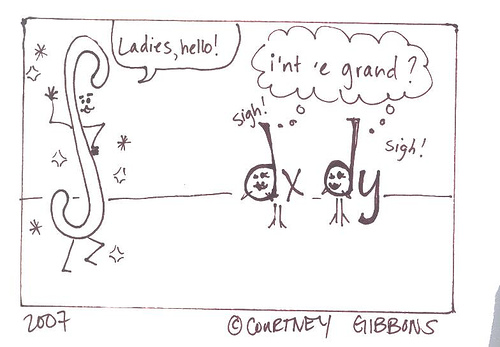
\includegraphics[width=4in]{integrand}
\end{center}

\noi If you were trying to find the area of a rectangle or in a trapezoid,
you would have no problem.  But what if you were trying to find the
area under a curve like this?


\begin{center}
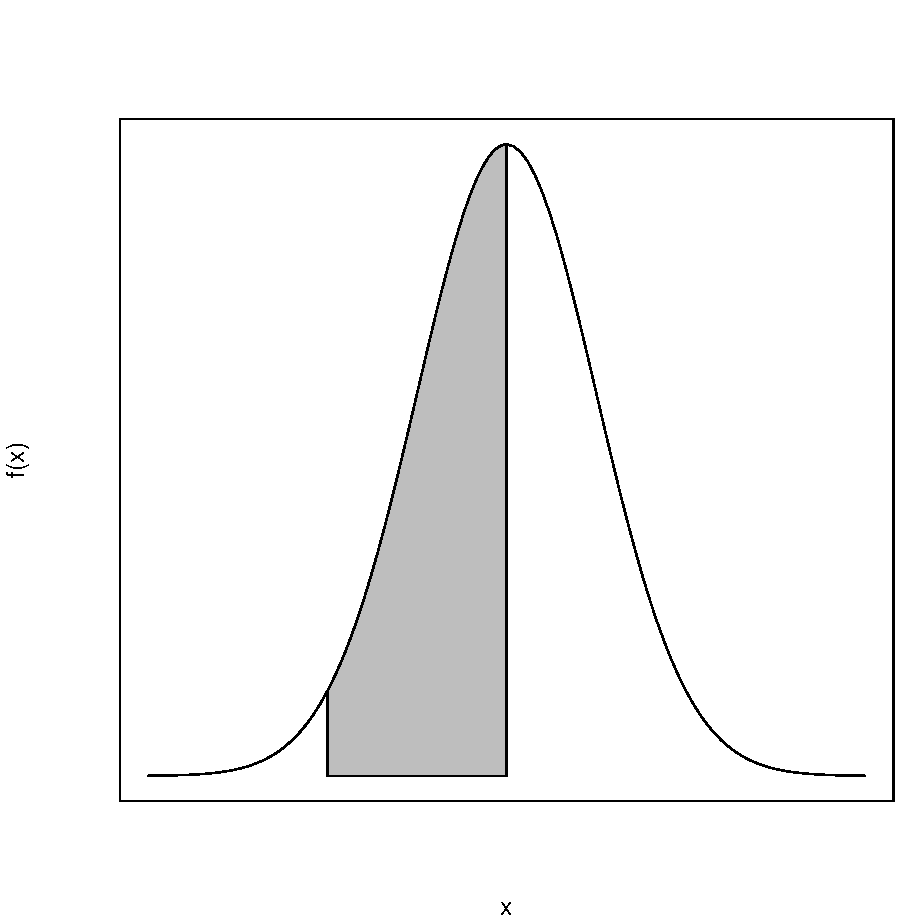
\includegraphics[width=2in]{Area}
\end{center}

\noi This is an important question, because the above function is a
drawing of the normal distribution -- the most commonly used
probability function in all of statistics.  The above picture is
essentially asking the question: what is the probability (i.e., $f(x)$)
of observing a value of $x$ between $-2$ and $0$?  

The answer, as it turns out, is sometimes very difficult to get.
Nonetheless it is very important.  You will be doing \textit{a lot} of
integration in statistics (especially if you venture into Bayesian
statistics).    And there are many, many applications of this
technique in game theory.  But in general, you will \textit{always} be
using these techniques for one of these two goals:
\bi
\item Finding the area under a curve
\item Finding a function given its derivative.  
\ei 

\noi Be aware that integration is sometimes (usually?)  \textit{hard}.
Sometimes it is impossible.  There are many important functions (e.g.,
the normal probability density function) whose indefinite integral has
never been derived.  Bayesian statistics was held back for hundreds of
years by the difficulties of integrating until computational methods
such as MCMC were developed and refined in the 1990s that made it
possible to get answers without actually solving.  Don't expect
solutions to integrals to jump off of the page at you.  Focus on
understanding the basic concept, and starting develop a library of
``tricks'' that mathematicians frequently use to solve these kinds of
problems.
 

\subsection{The Indefinite Integral: The Antiderivative}
\bi
\item Sometimes we're interested in exactly the
reverse:  finding the function $f$ for which $g$ is its derivative.  We
refer to $f$ as the {\bf antiderivative} of $g$.

\item Let $DF$ be the derivative of $F$.  And let $DF(x)$ be the
derivative of $F$ evaluated at $x$.  Then the antiderivative is denoted
by $D^{-1}$ (i.e., the inverse derivative).  If $DF=f$, then
$F=D^{-1}f$.

\item {\bf Indefinite Integral}:  Equivalently, if $F$ is the
antiderivative of $f$, then $F$ is also called the
indefinite integral of $f$ and written $F(x)=\lint f(x)dx$.

\item Examples:
  \be
  \item $\lint \frac{1}{x^2}dx=-\frac{1}{x}+c$
  \item $\lint 3e^{3x}dx=e^{3x}+c$
  \item \pbt{$\lint (x^2-4) dx=\frac{1}{3}x^3-4x+c$}
      \pb{\,  {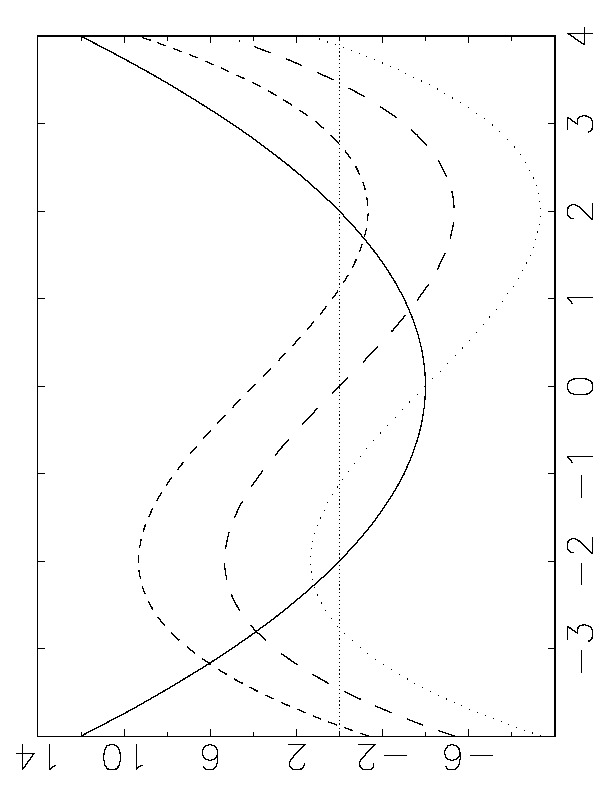
\includegraphics[width=1in, angle = 270]{derintegJ}}}
  \ee
\item Notice from these examples that while there is only a single
derivative for any function, there are multiple antiderivatives: one for
any arbitrary constant $c$.  $c$ just shifts the curve up or down on the
$y$-axis.  If more info is present about the antiderivative --- e.g.,
that it passes through a particular point --- then we can solve for a
specific value of $c$.

\item Common rules of integration:
  \be
  \item $\int a f(x)dx = a\int f(x)dx$
  \item $\int [f(x)+g(x)]dx=\int f(x)dx + \int g(x)dx$
  \item $\int x^n dx = \frac{1}{n+1} x^{n+1} + c $
  \item $\int e^x dx = e^x +c$
  \item $\int \frac{1}{x} dx = \ln x + c$
  \item $\int e^{f(x)}f'(x)dx = e^{f(x)}+c$
  \item $\int [f(x)]^n f'(x)dx = \frac{1}{n+1}[f(x)]^{n+1}+c$
  \item $\int \frac{f'(x)}{f(x)}dx=\ln f(x) + c$
  \ee

\item Examples:
  \be
  \item $\int 3x^2 dx= 3 \int x^2 dx = 3 \left( \frac{1}{3} x^3 \right)
+c= x^3 + c$
  \item $\int (2x+1)dx= \int 2x dx + \int 1 dx = x^2 + x +c $
  \item $\int e^x e^{e^x} dx = e^{e^x} + c$
  \ee
\ei

\subsection{The Definite Integral: The Area under the Curve}

\bi

\item {\bf Riemann Sum}:  Suppose we want to determine the area $A(R)$
of a region $R$ defined by a curve $f(x)$ and some interval $a\le x \le
b$.  One way to calculate the area would be to divide the interval $a\le
x\le b$ into $n$ subintervals of length $\Delta x$ and then approximate
the region with a series of rectangles, where the base of each rectangle
is $\Delta x$ and the height is $f(x)$ at the midpoint of that interval.
 $A(R)$ would then be approximated by the area of the union of the
rectangles, which is given by $$S(f,\Delta x)=\sum\limits_{i=1}^n
f(x_i)\Delta x$$ and is called a Riemann sum.

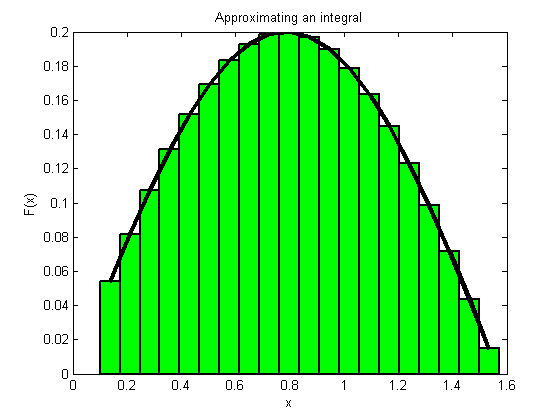
\includegraphics{riemann}

\item As we decrease the size of the subintervals $\Delta x$, making the
rectangles ``thinner," we would expect our approximation of the area of
the region to become closer to the true area.  This gives the limiting
process $$A(R)=\llim_{\Delta x\to 0}\sum\limits_{i=1}^n f(x_i)\Delta x$$

\item {\bf Riemann Integral}:  If for a given function $f$ the Riemann
sum approaches a limit as $\Delta x \to 0$, then that limit is
called the Riemann integral of $f$ from $a$ to $b$.  Formally,
$$\lint_a^b f(x) dx= \llim_{\Delta x\to 0}
\sum\limits_{i=1}^n f(x_i)\Delta x$$

\item {\bf Definite Integral}: We use the notation $\lint_a^b f(x) dx$
to denote the definite integral of $f$ from $a$ to $b$.  In words, the
definite integral $\lint_a^b f(x)dx$ is the area under the ``curve" f(x)
from $x=a$ to $x=b$.

\item {\bf First Fundamental Theorem of Calculus}:  Let the function $f$
be bounded on $[a,b]$ and continuous on $(a,b)$.  Then the function
$$F(x)=\lint_a^x f(s)ds, \quad a\le x\le b$$ has a derivative at each
point in $(a,b)$ and $$F'(x)=f(x), \quad a<x<b$$  This last point shows
that differentiation is the inverse of integration.

\item {\bf Second Fundamental Theorem of Calculus}:  Let the function
$f$ be bounded on $[a,b]$ and continuous on $(a,b)$.  Let $F$ be any
function that is continuous on $[a,b]$ such that $F'(x)=f(x)$ on
$(a,b)$.  Then $$\lint_a^bf(x)dx = F(b)-F(a)$$

\item Procedure to calculate a ``simple" definite integral $\lint_a^b
f(x)dx$:
  \be
  \item Find the indefinite integral $F(x)$.
  \item Evaluate $F(b)-F(a)$.
  \ee

\item Examples:
  \be
  \item $\lint_1^3 3x^2 dx=  \left. 3\left(\frac{1}{3} x^3\right) \right|_1^3 =
  (3)^3-(1)^3=26$
  \item $\lint_{-2}^2 e^x e^{e^x} dx = \left. e^{e^x} \right|_{-2}^2 =
  e^{e^{2}} -e^{e^{-2}}=1617.033 $
  \ee

\item Properties of Definite Integrals:
  \be
  \item \pbt{$\lint_a^a f(x)dx=0$}\pbff{There is no area below a point.}
  \item \pbt{$\lint_a^b f(x)dx=-\lint_b^a f(x)dx$}\pbff{Reversing the
limits changes the sign of the integral.}
  \item $\lint_a^b [\alpha f(x)+\beta g(x)]dx = \alpha \lint_a^b f(x)dx
+ \beta \lint_a^b g(x)dx$
  \item $\lint_a^b f(x) dx +\lint_b^c f(x)dx = \lint_a^c f(x)dx$
  \ee

\item Examples:
  \be
  \item $\lint_1^1 3x^2 dx = \left. x^3 \right|_1^1 =
 (1)^3-  (1)^3=0$
  \item $\lint_0^4 (2x+1)dx= 2\lint_0^4 x dx + \lint_0^4 1 dx =
\left. x^2 \right|_0^4 +\left. x \right|_0^4 = (16-0)+(4-0)=20 $
  \item $\lint_{-2}^0 e^x e^{e^x} dx + \lint_0^2 e^x e^{e^x} dx =
  \left. e^{e^x} \right|_{-2}^0 + \left. e^{e^x} \right|_{0}^2 =
  e^{e^{0}} -e^{e^{-2}} + e^{e^{2}} -e^{e^{0}}=
  e^{e^{2}} -e^{e^{-2}}=1617.033 $
  \ee

\ei

\subsection{Integration by Substitutions}
\bi

\item Sometimes the integrand doesn't appear integrable using common
rules and antiderivatives.  A method one might try is {\bf integration
by substitutions}, which is related to the Chain Rule.

\item Suppose we want to find the indefinite integral $\int g(x)dx$ and
assume we can identify a function $u(x)$ such that $g(x)=f[u(x)]u'(x)$.
Let's refer to the antiderivative of $f$ as $F$.  Then the chain rule
tells us that $\frac{d}{dx} F[u(x)]=f[u(x)]u'(x)$.  So, $F[u(x)]$ is the
antiderivative of $g$.  We can then write $$\int g(x) dx= \int
f[u(x)]u'(x)dx = \int \frac{d}{dx} F[u(x)]dx = F[u(x)]+c$$

\item Procedure to determine the indefinite integral $\int g(x)dx$ by
the method of substitutions:
  \be
  \item Identify some part of $g(x)$ that might be simplified by
substituting in a single variable $u$ (which will then be a function of
$x$).
  \item Determine if $g(x)dx$ can be reformulated in terms of $u$ and
$du$.
  \item Solve the indefinite integral.
  \item Substitute back in for $x$
  \ee

\item Substitution can also be used to calculate a definite integral.
Using the same procedure as above, $$\lint_a^b g(x)dx=\lint_c^d f(u)du =
F(d)-F(c)$$ where $c=u(a)$ and $d=u(b)$.

\item Examples:
  \be
  \item $\int x^2 \sqrt{x+1}dx$\\[6pt]
  The problem here is the $\sqrt{x+1}$ term.  However, if the integrand
had $\sqrt{x}$ times some polynomial, then we'd be in business.  Let's
try $u=x+1$.  Then $x=u-1$ and $dx=du$.  Substituting these into the
above equation, we get
\beqa
\int x^2\sqrt{x+1}dx&=&\int (u-1)^2\sqrt{u}du\non\\
                    &=&\int (u^2-2u+1)u^{1/2}du\non\\
                    &=&\int (u^{5/2}-2u^{3/2}+u^{1/2})du\non
\eeqa
We can easily integrate this, since it's just a polynomial.  Doing so
and substituting $u=x+1$ back in, we get $$\int
x^2\sqrt{x+1}dx=2(x+1)^{3/2}\left[\frac{1}{7}(x+1)^2 -
\frac{2}{5}(x+1)+\frac{1}{3}\right]+c$$
  \item For the above problem, we could have also used the substitution
$u=\sqrt{x+1}$.  Then $x=u^2-1$ and $dx=2u du$.  Substituting these in,
we get $$\int x^2\sqrt{x+1}dx=\int (u^2-1)^2 u 2u du$$ which when
expanded is again a polynomial and gives the same result as above.

  \item $\lint_0^1 \frac{5e^{2x}}{(1+e^{2x})^{1/3}}dx$\\[6pt]
  When an expression is raised to a power, it's often helpful to use
this expression as the basis for a substitution.  So, let $u=1+e^{2x}$.
Then $du=2e^{2x}dx$ and we can set $5e^{2x}dx=5du/2$.    Additionally, $u=2$
when $x=0$ and $u=1+e^2$ when $x=1$.  Substituting all of this in, we
get
\beqa
\lint_0^1 \frac{5e^{2x}}{(1+e^{2x})^{1/3}}dx
    &=& \frac{5}{2}\lint_2^{1+e^2}\frac{du}{u^{1/3}}\non\\
    &=& \frac{5}{2}\lint_2^{1+e^2} u^{-1/3}du\non\\
    &=& \left. \frac{15}{4} u^{2/3} \right|_2^{1+e^2}\non\\
    &=& 9.53\non
\eeqa
  \ee

\ei

\subsection{Integration by Parts} \bi \item Another useful integration
technique is {\bf integration by parts}, which is related to the Product
Rule of differentiation. The product rule states that
$$\frac{d}{dx}(uv)=u\frac{dv}{dx}+v\frac{du}{dx}$$  Integrating this and
rearranging, we get $$\int u\frac{dv}{dx}dx= u v - \int v
\frac{du}{dx}dx$$ or $$\int u(x) v'(x)dx=u(x)v(x) - \int v(x)u'(x)dx$$
More frequently remembered as $$\int u dv = u v - \int v
du$$ where $du=u'(x)dx$ and $dv=v'(x)dx$.

\item For definite integrals: $\lint_a^b
u\frac{dv}{dx}dx = \left. u v \right|_a^b - \lint_a^b v
\frac{du}{dx}dx$

\item Our goal here is to find expressions for $u$ and $dv$ that, when
substituted into the above equation, yield an expression that's more
easily evaluated.

\item Examples:
  \be
  \item $\int x e^{ax} dx$\\[6pt]
  Let $u=x$ and $dv=e^{ax}dx$.  Then $du=dx$ and $v=(1/a)e^{ax}$.
Substituting this into the integration by parts formula, we obtain
\beqa
\int x e^{ax} dx &=& u v - \int v du\non\\
         &=&x\left( \frac{1}{a}e^{ax}\right) -
            \int\frac{1}{a}e^{ax}dx\non\\
         &=&\frac{1}{a}xe^{ax}-\frac{1}{a^2}e^{ax}+c\non
\eeqa
   \item $\int x^n e^{ax} dx$\\[6pt]
   As in the first problem, let's let $u=x^n$ and $dv=e^{ax}dx$.  Then
$du=n x^{n-1}dx$ and $v=(1/a)e^{ax}$.  Substituting these into the
integration by parts formula gives
\beqa
\int x^n e^{ax} dx &=& u v - \int v du\non\\
         &=&x^n\left( \frac{1}{a}e^{ax}\right) -
            \int\frac{1}{a}e^{ax} n x^{n-1} dx\non\\
         &=&\frac{1}{a}x^n e^{ax} -
             \frac{n}{a}\int x^{n-1}e^{ax}dx\non
\eeqa
Notice that we now have an integral similar to the previous one, but
with $x^{n-1}$ instead of $x^n$.  For a given $n$, we would repeat the
integration by parts procedure until the integrand was directly
integrable --- e.g., when the integral became $\int e^{ax}dx$.\\

  \item $\int x^3 e^{-x^2} dx$\\[6pt]
  We could, as before, choose $u=x^3$ and $dv=e^{-x^2}dx$.  But we
can't then find $v$ --- i.e., integrating $e^{-x^2}dx$ isn't possible.
Instead, notice that $d(e^{-x^2})/dx=-2xe^{-x^2}$, which can be factored
out of the original integrand $$\int x^3 e^{-x^2} dx = \int x^2
(xe^{-x^2})dx$$  We can then let $u=x^2$ and $dv=x e^{-x^2}dx$.  Then
$du=2x dx$ and $v=-\frac{1}{2}e^{-x^2}$.  Substituting these in, we have
\beqa
\int x^3 e^{-x^2} dx &=& u v - \int v du\non\\
             &=& x^2 \left( -\frac{1}{2}e^{-x^2}\right)
                 -\int \left(-\frac{1}{2}e^{-x^2}\right)2x dx\non\\
             &=& -\frac{1}{2}x^2 e^{-x^2}+\int x e^{-x^2}dx\non\\
             &=& -\frac{1}{2}x^2 e^{-x^2}-\frac{1}{2}e^{-x^2}+c\non
\eeqa
and the rest is algebra.

  \ee

\ei

\section{Calculus with a matrix}

\begin{center}
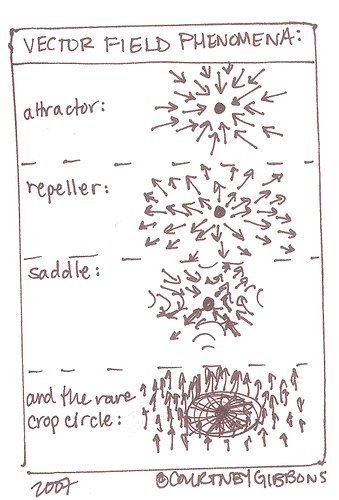
\includegraphics[width=3in]{signs}
\end{center}

This is where things get cool (but also a bit tricky).  Just like we
often have too many equations and variables to deal with efficiently
in pieces for basic algebraic operations, we will often want a better
way to do calculus.  In these situations, very smart people have
developed matrix methods for handling differentiation equivalent to
first (gradients) and second (Hessians) derivatives.  This is pretty
useful for finding global maxima and minimum in multi-dimensional
spaces.  

Unfortunately, there aren't a set of equally clean methods for dealing
with multidimensional integration.  That's good news for you today
(since you don't have to learn about it), but bad news for the rest of
your life since you will spend a lot of your time working with
imperfect numerical approximations of high-dimensional integrals.


\subsection{Differentiation in several variables}
\bi
\item Suppose we have a function $f$ now of two (or more) variables and we
want to determine the rate of change relative to one of the variables.
To do so, we would find its partial derivative, which is defined
similar to the derivative of a function of one variable.

\item {\bf Partial Derivative}:  Let $f$ be a function of the variables
$(x_1,\ldots,x_n)$.  The partial derivative of $f$ with respect to $x_i$
is $$\frac{\partial f}{\partial x_i} (x_1,\ldots,x_n) =
\llim_{h\to 0}
\frac{f(x_1,\ldots,x_i+h,\ldots,x_n)-f(x_1,\ldots,x_i,\ldots,x_n)}{h}$$
Only the $i$th variable changes --- the others are treated as constants.

\item We can take higher-order partial derivatives, like we did with
functions of a single variable, except now we the higher-order partials
can be with respect to multiple variables.

\item Examples:
  \be
  \item $f(x,y)=x^2+y^2$\\
  $\frac{\partial f}{\partial x}(x,y)=2x$\\
  $\frac{\partial f}{\partial y}(x,y)=2y$\\
  $\frac{\partial^2 f}{\partial x^2}(x,y)=2$\\
  $\frac{\partial^2 f}{\partial x \partial y}(x,y)=0$
  \item $f(x,y)=x^3 y^4 +e^x -\ln y$\\
  $\frac{\partial f}{\partial x}(x,y)=3x^2 y^4 +e^x$\\
  $\frac{\partial f}{\partial y}(x,y)=4x^3y^3-1/y$\\
  $\frac{\partial^2 f}{\partial x^2}(x,y)=6xy^4+e^x$\\
  $\frac{\partial^2 f}{\partial x \partial y}(x,y)=12x^2y^3$
  \ee

\ei


\subsection{Integration with several variables}

\bi

\item Now suppose we want to reverse the process.  Say we have a function
$f$ now of two (or more) variables and we want to determine the area
under the surface (or hypersurface).

Take the total function and choose one of the variables (although you
will want to be strategic about this choice).  Perform the
integration, while \textit{treating the other variable as a constant}.
Make sure you keep track of the ${\partial x_i}$ symbols.

$$\lint \lint (2x+2y) {\partial x}{\partial y} = \lint x^2 + 2xy {\partial y} + c $$
$$ = yx^2 + xy^2 + ?$$

\item This is not as straight-forward as it seems because indefinite
  integrals are only correct up to a constant.  For instance:

$$\lint x^3 = \frac{1}{4}x^4 + 10 $$
or
$$=\frac{1}{4}x^4 - 10$$
or (if we are treating $y$ as a constant)
$$=\frac{1}{4}x^4 - e^y$$

\item Likewise:

$$\lint \lint 12x^2y^3 {\partial x}{\partial y}$$
$$= x^3y^4 + e^x - ln(y)$$
or
$$=x^3y^4 + 24x-y^{monkey}$$


\item Usually we get around this by making use of the fact that we
  know that function we are working with integrates to a known
  constant or when the integrated function passes through a specific
  point.  For instance, we know that any probability function must
  integrate to 1.  But often, even this doesn't help that much when we
  are integrating many times across many dimensions.

\item None of this is particularly important for anything you will be
  doing soon.  Just something to keep in mind as you work towards more
  advanced methods.

\ei



\subsection{Vector representation of calculus}

\bi

\item The function $y = f(x_1, x_2, \ldots,x_n)$ of the independent variable
$x_1, x_2, \ldots, x_n$ can be written as the function $y=f({\bf
  x})$ where ${\bf x} = (x_1, x_2, \ldots, x_n)'$.  

\item The \textbf{gradient} is the vector of partial derivatives and is
  denoted:

$$\grad = \bpm
\frac{\pf}{\pr x_1}\\[9pt] \frac{\pf}{\pr x_2}\\
  \vdots \\[3pt] \frac{\pf}{\pr x_n} \epm$$



\item The  {\bf Hessian} $\hx$ is
an $n\times n$ matrix, where the $(i,j)$th element is the second order
partial derivative of $f(\bfx)$ with respect to $x_i$ and $x_j$:
$$\hx=\bpm
\frac{\pr^2 \fx}{\pr x_1^2}&\frac{\pr^2\fx}{\pr x_1 \pr x_2}&
\cdots & \frac{\pr^2 \fx}{\pr x_1 \pr x_n}\\[9pt]
\frac{\pr^2 \fx}{\pr x_2 \pr x_1}&\frac{\pr^2\fx}{\pr x_2^2}&
\cdots & \frac{\pr^2 \fx}{\pr x_2 \pr x_n}\\
\vdots & \vdots & \ddots & \vdots \\[3pt]
\frac{\pr^2 \fx}{\pr x_n \pr x_1}&\frac{\pr^2\fx}{\pr x_n \pr x_2}&
\cdots & \frac{\pr^2 \fx}{\pr x_n^2}\epm$$


\ei


\subsection{Maxima and Minima in $\rn$}

\bi

\item {\bf Conditions for Extrema}:  The conditions for extrema are
similar to those for functions on $\ro$.  Let $f(\bfx)$ be a function of
$n$ variables.  Let $B(\bfx, \eps)$ be the $\eps$-ball about the point
$\bfx$.  Then
  \be
  \item \pbt{$f(\bfx^*)>f(\bfx), \: \forall \bfx\in B(\bfx^*,\eps)$}
  $\qquad \lra \qquad$ Strict Local Max
  \item \pbt{$f(\bfx^*)\ge f(\bfx), \: \forall \bfx\in B(\bfx^*,\eps)$}
  $\qquad \lra \qquad$ Local Max
  \item \pbt{$f(\bfx^*)<f(\bfx), \: \forall \bfx\in B(\bfx^*,\eps)$}
  $\qquad \lra \qquad$ Strict Local Min
  \item \pbt{$f(\bfx^*)\le f(\bfx), \: \forall \bfx\in B(\bfx^*,\eps)$}
  $\qquad \lra \qquad$ Local Min
  \ee
\ei

\subsection{First Order Conditions}
\bi
\item When we examined functions
of one variable $x$, we found critical points by taking the first
derivative,  setting it to zero, and solving for $x$.  For functions of
$n$ variables, the critical points are found in much the same way,
except now we set the partial derivatives equal to zero.\footnote{We
will only consider critical points on the interior of a function's
domain.}

\item $\bfx^*$ is a critical point iff $\nabla f(\bfx^*)=0$.

\item Example: Find the critical points of $\fx=(x_1-1)^2+x_2^2+1$
  \be
  \item The partial derivatives of $\fx$ are
  \beqa
  \frac{\pf}{\pr x_1}&=&2(x_1-1)\non\\
  \frac{\pf}{\pr x_2}&=&2x_2\non
  \eeqa
  \item Setting each partial equal to zero and solving for $x_1$ and
$x_2$, we find that there's a critical point at $\bfx^*=(1,0)$.
  \ee
\ei

\subsection{Second Order Conditions}
\bi
\item When we found a critical point for
a function of one variable, we used the second derivative as an
indicator of the curvature at the point in order to determine whether
the point was a min, max, or saddle.  For functions of $n$ variables, we
 use second order partial derivatives as an indicator of curvature.

\newcommand{\bfh}{{\bf h}}
\item {\bf Curvature and The Taylor Polynomial as a Quadratic Form}:
The Hessian is used in a Taylor polynomial approximation to $\fx$ and
provides information about the curvature of $\fx$ at $\bfx$ --- e.g., which
tells us whether a critical point $\bfx^*$ is a min, max, or saddle point.
  \be
  \item The second order Taylor polynomial about the critical point
$\bfx^*$ is
  $$f(\bfx^*+\bfh)=f(\bfx^*)+\nabla f(\bfx^*) \bfh +\frac{1}{2} \bfh^T
{\bf H(x^*)} \bfh + R(\bfh)$$
  \item Since we're looking at a critical point, $\nabla f(\bfx^*)=0$;
and for small $\bfh$, $R(\bfh)$ is negligible.  Rearranging, we get
$$f(\bfx^*+\bfh)-f(\bfx^*)\approx \frac{1}{2} \bfh^T {\bf H(x^*)}
\bfh $$
  \item The RHS is a quadratic form and we can determine the definiteness of $\bf
H(x^*)$.\\
    \be
    \item If $\bf H(x^*)$ is positive definite, then the RHS is positive
for all small $\bfh$:
$$f(\bfx^*+\bfh)-f(\bfx^*)>0 \quad\lra\quad f(\bfx^*+\bfh)>f(\bfx^*)$$
i.e., $f(\bfx^*)<f(\bfx), \: \forall \bfx\in B(\bfx^*,\eps)$, so
$\bfx^*$ is a strict local min.\\
    \item Conversely, if $\bf H(x^*)$ is negative definite, then the RHS
is negative for all small $\bfh$:
$$f(\bfx^*+\bfh)-f(\bfx^*)<0 \quad\lra\quad f(\bfx^*+\bfh)<f(\bfx^*)$$
i.e., $f(\bfx^*)>f(\bfx), \: \forall \bfx\in B(\bfx^*,\eps)$, so
$\bfx^*$ is a strict local max.\\
    \ee
  \ee

\smallskip

\item {\bf Summary of Second Order Conditions}:\\[6pt]
Given a function $\fx$ and a point $\bfx^*$ such that $\nabla
f(\bfx^*)=0$,
  \be
  \item \pbt{$\bf H(x^*)$ Positive Definite} $\quad \lra \quad$
  Strict Local Min
  \item \pbt{$\bf H(x)$ Positive Semidefinite\\ $\forall \bfx\in
B(\bfx^*,\eps)$} $\quad \lra \quad$
  Local Min
  \item \pbt{$\bf H(x^*)$ Negative Definite} $\quad \lra \quad$
  Strict Local Max
  \item \pbt{$\bf H(x)$ Negative Semidefinite\\ $\forall \bfx\in
B(\bfx^*,\eps)$} $\quad \lra \quad$
  Local Max
  \item \pbt{$\bf H(x^*)$ Indefinite} $\quad \lra \quad$
  Saddle Point
  \ee

\smallskip

\item Example:  We found that the only critical point of
$\fx=(x_1-1)^2+x_2^2+1$ is at $\bfx^*=(1,0)$.  Is it a min, max, or
saddle point?
  \be
  \item Recall that the gradient of $\fx$ is
  $$\grad = \bpm
  2(x_1-1)\\
  2x_2 \epm$$
  Then the Hessian is
  $$\bf H(\bfx)=\bpm 2&0\\0&2 \epm$$
  \item To check the definiteness of $\bf H(\bfx^*)$, we could use
either of two methods:
    \be
    \item  Determine whether $\bf x^T H(\bfx^*) x$ is greater or less
than zero for all $\bf x\ne 0$:
$${\bf x^T H(\bfx^*) x} = \bpm x_1 & x_2 \epm \bpm 2&0\\0&2 \epm
\bpm x_1\\x_2\epm = 2x_1^2+2x_2^2$$
For any $\bf x\ne 0$, $2(x_1^2+x_2^2)>0$, so the Hessian is positive
definite and $\bfx^*$ is a strict local minimum.
    \item Using the method of leading principal minors, we see that
$M_1=2$ and $M_2=4$.  Since both are positive, the Hessian is positive
definite and $\bfx^*$ is a strict local minimum.
    \ee
  \ee

\item Does this seem confusing?  What it mean for a matrix to be
  ``definite''?  

\ei

\subsection{Redux: Definiteness}

\bi

\item \textbf{A positive definite matrix is always nonsingular}.  When
  you come across this term, it is usually there to specify that the
  matrix can be inverted, and a solution to some system of equations
  is possible.

\item When some $n \times n$ matrix  $\bfa$ is pre- and
  post-multiplied by a conformable non-zero matrix ${\bf x}$, we get
  the equation:

$${\bf x'}\bfa {\bf x}=c$$

\item Some properties of the quadratic.  For all nonzero vectors
  ${\bf x}$:
\bi
\item $\bfa$ is said to be \textbf{positive definite} if $c>0$.
\item $\bfa$ is said to be \textbf{positive semidefinite} if $c\ge0$.
\item $\bfa$ is said to be\textbf{ negative definite} if $c<0$.
\item $\bfa$ is said to be \textbf{negative semidefinite} if $c\le0$.
\ei

\item Examples:
  \be
  \item

\pbt{Positive Definite:\\

$ \begin{array}{rl}
Q(\bfx) &=\bfx^T \bpm 1&0\\0&1\epm \bfx \\
         &=x_1^2+x_2^2
\end{array} $ }
\parbox{2in}{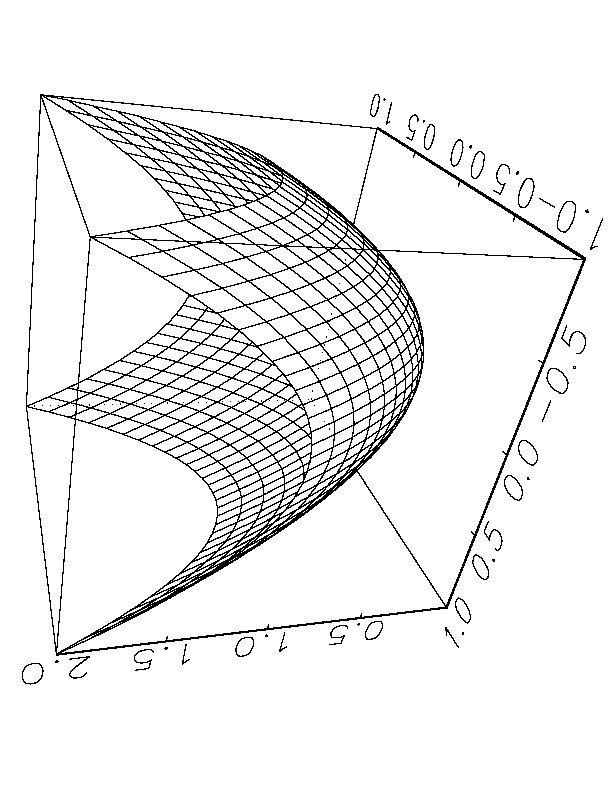
\includegraphics[angle=270, width=2.5in]{posdefJ}}

  \item \pbt{Positive Semidefinite:\\

$ \begin{array}{rl}
Q(\bfx)&=\bfx^T \bpm 1&-1\\-1&1\epm \bfx \\
       &=(x_1-x_2)^2
\end{array} $ }
\parbox{2in}{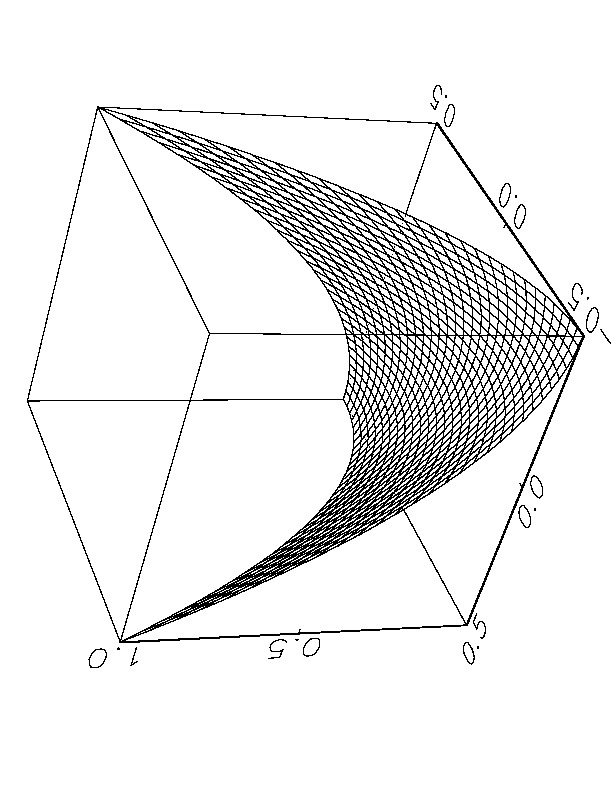
\includegraphics[angle=270, width=2.5in]{possemJ}}

  \item \pbt{Indefinite:\\

$ \begin{array}{rl}
Q(\bfx)&=\bfx^T \bpm 1&0\\0&-1\epm \bfx \\
       &=x_1^2-x_2^2
       \end{array} $ }
  \parbox{2in}{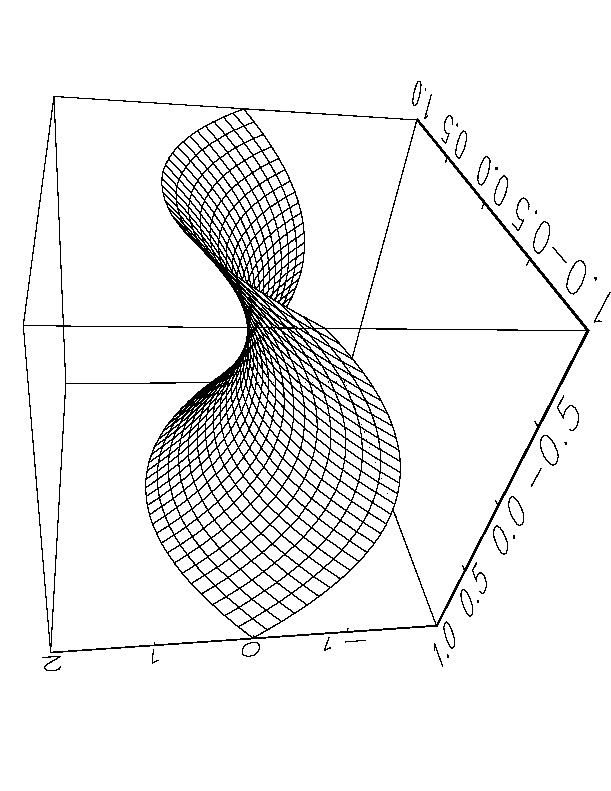
\includegraphics[angle=270, width=2.5in]{indefJ}}
  \ee



\ei

\subsection{Redux: Test for definiteness}
\bi

\item Given an $n\times n$ matrix $\bfa$, $k$th order {\bf principal
minors} are the determinants of the $k\times k$ submatrices along the
diagonal obtained by deleting $n-k$ columns and the same $n-k$ rows from
$\bfa$.

\item Example: For a $3\times 3$ matrix $\bfa$,
  \be
  \item First order principal minors:
$$|a_{11}|, \quad |a_{22}|, \quad |a_{33}|$$
  \item Second order principal minors:
$$ \bvm a_{11}&a_{12}\\a_{21}&a_{22}\evm, \quad
   \bvm a_{11}&a_{13}\\a_{31}&a_{33}\evm, \quad
   \bvm a_{22}&a_{23}\\a_{32}&a_{33}\evm$$
  \item Third order principal minor:  $|\bfa|$
  \ee

\item Define the $k$th {\bf leading principal minor} $M_k$ as the determinant
of the $k\times k$ submatrix obtained by deleting the last $n-k$ rows
and columns from $\bfa$.

\item Example: For a $3\times 3$ matrix $\bfa$, the three leading principal
minors are
$$M_1=|a_{11}|, \quad M_2=\bvm a_{11}&a_{12}\\a_{21}&a_{22}\evm, \quad
M_3=\bvm a_{11}&a_{12}&a_{13}\\
         a_{21}&a_{22}&a_{23}\\
         a_{31}&a_{32}&a_{33} \evm$$

\item Algorithm:  If $\bfa$ is an $n\times n$ symmetric matrix, then
  \be
  \item \pbt{$M_k>0, \: k=1,\ldots,n$} $\qquad \lra \qquad$ Positive
Definite
  \item \pbt{$M_k<0, \: \mbox{for odd  } k$ and\\
         $M_k>0, \: \mbox{for even } k$} $\qquad \lra \qquad$
Negative Definite
  \item \pbt{$M_k\ne 0, \: k=1,\ldots,n$,\\ but does not fit the pattern
of 1 or 2.} $\qquad \lra \qquad$ Indefinite.
  \ee

\item If some leading principal minor is zero, but all others fit the pattern
of the preceding conditions 1 or 2, then
  \be
  \item \pbt{Every principal minor $\ge 0$} $\qquad \lra \qquad$
Positive Semidefinite
  \item \pbt{Every principal minor of odd order $\le 0$ and
  every principal minor of even order $\ge 0$} $\qquad \lra \qquad$
Negative Semidefinite
  \ee

\ei


\subsection{Global maxima and minima}
\bi

\item To determine whether a critical point is a global min or max, we
can check the concavity of the function over its entire domain.  Here
again we use the definiteness of the Hessian to determine whether a
function is globally concave or convex:
  \be
  \item \parbox[t]{2.3in}{$\bf H(x)$ Positive Semidefinite $\forall \bfx$} $\quad
\lra \quad$ Globally Convex
  \item \parbox[t]{2.3in}{$\bf H(x)$ Negative Semidefinite $\forall \bfx$} $\quad
\lra \quad$ Globally Concave
  \ee
Notice that the definiteness conditions must be satisfied over the
entire domain.

\item Given a function $\fx$ and a point $\bfx^*$ such that $\nabla
f(\bfx^*)=0$,
  \be
  \item \pbt{$\fx$ Globally Convex} $\quad
\lra \quad$ Global Min
  \item \pbt{$\fx$ Globally Concave} $\quad
\lra \quad$ Global Max
  \ee

\item Note that showing that $\bf H(x^*)$ is negative semidefinite is
not enough to guarantee $\bfx^*$ is a local max.  However, showing that
$\bf H(x)$ is negative semidefinite for all $\bfx$ guarantees that $x^*$
is a global max.  (The same goes for positive semidefinite and minima.)

\item Example: Take $f_1(x)=x^4$ and $f_2(x)=-x^4$.  Both have $x=0$ as
a critical point.  Unfortunately, $f''_1(0)=0$ and $f''_2(0)=0$, so we
can't tell whether $x=0$ is a min or max for either.  However,
$f''_1(x)=12x^2$ and $f''_2(x)=-12x^2$.  For all $x$, $f''_1(x)\ge 0$
and $f''_2(x)\le 0$ --- i.e., $f_1(x)$ is globally convex and $f_2(x)$
is globally concave.  So $x=0$ is a global min of $f_1(x)$ and a
global max of $f_2(x)$.

\ei


\subsection{Example (thanks Harvard!)}
\bi
\item Given $f(\bfx)=x_1^3-x_2^3+9x_1x_2$, find any maxima or minima.
  \be
  \item First-order conditions.  Set the gradient equal to zero and
solve for $x_1$ and $x_2$.
  \beqa
  \frac{\pr f}{\pr x_1}&=&3x_1^2+9x_2=0\non\\
  \frac{\pr f}{\pr x_2}&=&-3x_2^2+9x_1=0\non
  \eeqa
  We have two equations in two unknowns.  Solving for $x_1$ and $x_2$,
we get two critical points:  $\bfx_1^*=(0,0)$ and $\bfx_1^*=(3,-3)$.
  \item Second order conditions.  Determine whether the Hessian is
positive or negative definite.  The Hessian is
  $$\bf H(x)=\bpm 6x_1&9\\9&-6x_2 \epm$$
  Evaluated at $\bfx_1^*$, $$\bf H(x_1^*)=\bpm 0&9\\9&0\epm$$  The two leading
principal minors are $M_1=0$ and $M_2=-81$, so $\bf H(x_1^*)$ is
indefinite and $\bfx_1^*=(0,0)$ is a saddle point.\\[9pt]
  Evaluated at $\bfx_2^*$, $$\bf H(x_2^*)=\bpm 18&9\\9&18\epm$$   The
two leading principal minors are $M_1=18$ and $M_2=243$.  Since both are
positive, $\bf H(x_2^*)$ is positive definite and $\bfx_2^*=(3,-3)$ is a
strict local min.
  \item Global concavity/convexity.  In evaluating the Hessians for
$\bfx_1^*$ and $\bfx_2^*$ we saw that the Hessian is not everywhere
positive semidefinite.  Hence, we can't infer
that $\bfx_2^*=(3,-3)$ is a global minimum.  In fact, if we set $x_1=0$,
the $f(\bfx)=-x_2^3$, which will go to $-\infty$ as $x_2\to \infty$.
  \ee
\ei



\end{document}


Advanced Counting
- Combinations
- permutations
- ordered and unordered
- Replacement
- Finite and infinite series

Sets
- Sets
- Special properties of sets
- Special sets
-  Set operations
- Properties for three sets

Probabilities
- Probability Functions
- Conditional probabilities and Bayes Law
- Independence
- Odds and probabilities


Measures

Distribution Functions
- pmf
-pdf
-cdf
- specifics

Moments (Theoretical measures of centrality/spread)

Correlation and covariance